\documentclass[10pt,a4paper]{report}
\usepackage[T1]{fontenc}
\usepackage[width=16cm, height=27cm]{geometry}
\usepackage{color}
\usepackage{pdfpages}
\usepackage{graphicx}
\usepackage{wrapfig}
\title{Abschlussarbeit}
\author{Benjamin Schulze}
\begin{document}
	\begin{titlepage}
		\begin{flushleft}
			
\includegraphics[scale=0.3]{HTWK_Logo.jpg}
		\end{flushleft}
		
		\begin{flushright}
			\vspace{2cm}
			\LARGE \textsl{Aufbauanleitung} \\
			\rule{0.6\textwidth}{0.4pt} ~\\
			\vspace{0.5cm}
			\textsf{\LARGE Cocktailmaschine}
		\end{flushright}
		
		\vspace{3cm}
		\large
		\begin{tabbing}
			xxxxxxxxxxxxxxxxxxxxxxx \= \kill
			Autor: \> Benjamin Schulze, Aicha El Goufri, Huy Phan, \\\>Max Vinzens, Leon Arnecke und Elvira Lüders \\ [0.5cm]
			Studiengang:  \> Elektro- und Informationstechnik \\ [0.5cm]
			Modul:  \> Ausgewählte Themen der Automatisierungstechnik \\ [0.5cm]
			Stand: \> 18.09.2023 \\
		\end{tabbing}
		
		\vspace{4cm}
		\small
		\begin{center}
			Hochschule für Technik, Wirtschaft und Kultur Leipzig \\$\cdot$
			Fakultät Ingenieurwissenschaften $\cdot$
			Abteilung MSR \\
			Karl-Liebknecht-Straße 132 $\cdot$
			04277 Leipzig $\cdot$
			https://www.htwk-leipzig.de
		\end{center}
	\end{titlepage}
	\newpage
	\tableofcontents
	
	\chapter{Einleitung}
	Dies ist die Aufbauanleitung für die im Modul "Ausgewählte Themen der Automatisierungstechnik" erstellte Cocktailmaschine.
	
	\chapter{Materialliste}
	\section{Material und Hardware}
	Gehäuse
	- 4x Profilschiene (3x3 cm) 70cm\\
	- 8x Profilschiene (3x3 cm) 28cm\\
	- 6x Winkel\\
	- 2x Holzbrett 70 x 28 cm\\ 
	- 2x Holzbrett 64 x 28 cm\\
	- diverse Schrauben und Nutensteine\\
	Verschlauchung
	- 8x Leerkanister aus HD-PE\\
	- 8x Ventil\\
	- 1x Schlauch (6mm Lebensmittelecht) 15 m\\
	- 8x Fittings ( ½ Zoll (DN 15) Innengewinde auf 6mm Innendurchmesser Schlauch)\\
	- 8x Fitting ( Schlauchverbinder 10 mm auf 6 mm)\\
	- 7x T Stücke (6mm)\\
	- 1x Pumpe\\
	- 16x Verschraubung (M16X1,5)\\
	- 9x Schlauchschellen\\
	- 1x Schlauch (10mm Lebensmittelecht) 0,5 m\\
	
	- 1x Netwerkkabel \\
	- 1x Hohlteckerkabel\\
		
		
	\section{3D gedrucktes Material}
	Die folgenden Objekte aus dem Ordner Fusion bzw. 3d\_Druck sind vor Beginn zu fertigen.
	

	\chapter{Gehäuse}
	\section{Gehäuseaufbau}
	Unsere Cocktailmaschine hat ungefähr die Form eines Quaders (siehe Abb.1). Das Grundgehäuse besteht aus zwei Hauptmaterialien, Profilschienen (3x3 cm) aus Aluminium und den Außenwänden aus Holz. Die Profilschienen dienen als Grundskelett, um möglichst viel Stabilität zu erreichen. Vier senkrechte Träger mit einer Höhe von 70 cm und acht waagerechte Träger (vier oben, vier unten, von denen jeweils zwei gegenüberliegende um 3 cm höhenversetzt sind) von 28 cm Länge bilden zusammen die quaderähnliche Form (siehe Abb.2). Zwei weitere waagerechte Profilschienen auf 20 cm Höhe dienen zur weiteren Stabilisation. Diese sind vorne und hinten angebracht. Außerdem wird die Vordere dafür verwendet, die später anzubringende Wägezelle zu befestigen.
	Zum Befestigen der Profilschienen wird in das runde Loch im Querschnitt auf allen Seiten ein Gewinde gefräst. Dies betrifft ausschließlich die kurzen Profilschienen. In die langen Profilschienen werden von außen auf gleicher Höhe wie die Gewinde (bei 3x3 cm dicken Profilschienen ist das mittige Gewinde auf 1,5cm Höhe) Löcher gebohrt, sodass man alle Profilschienen miteinander verbinden kann (siehe Abb.2).  
	
\begin{figure}[htb]
	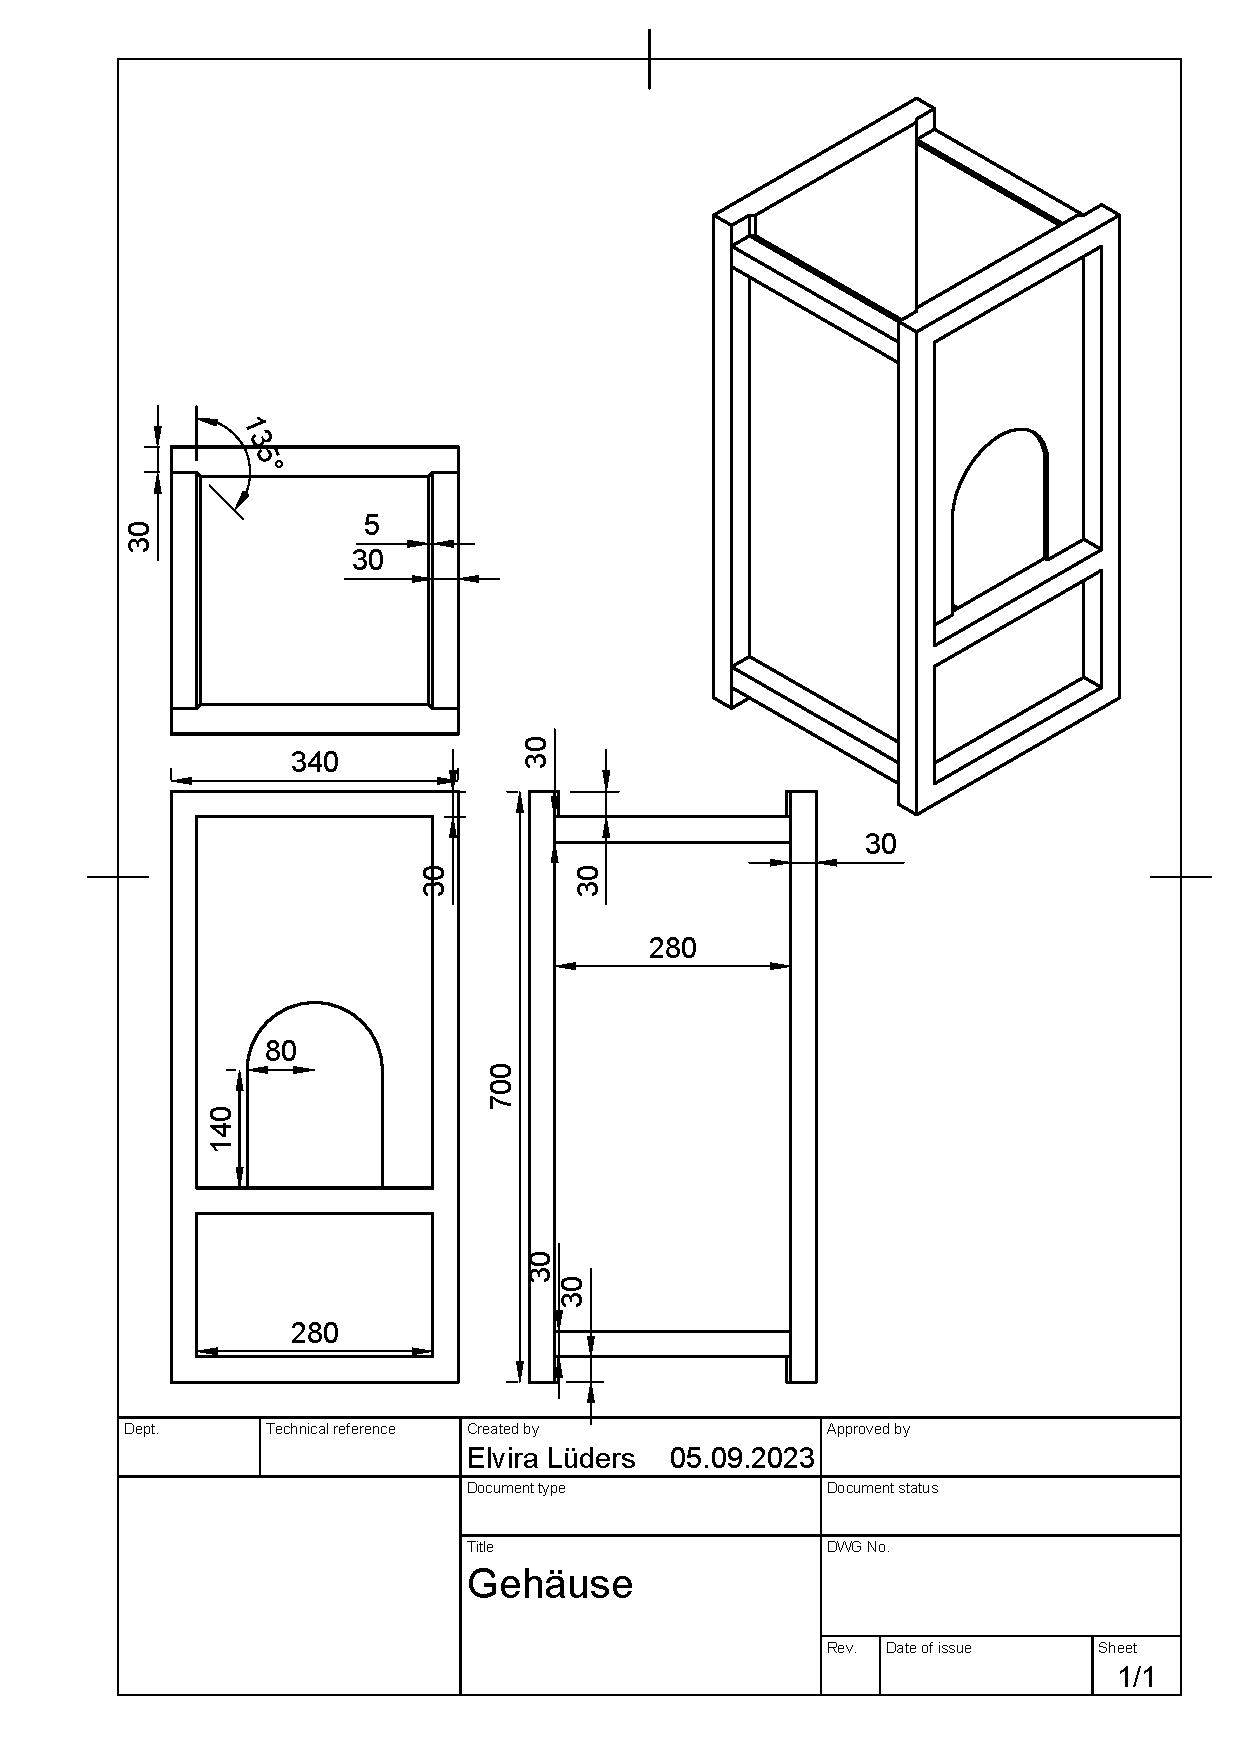
\includegraphics[width=0.5\textwidth]{Abb.8 Grundaufbau_Skizze.pdf}\\
	\centering
	\caption{Abb.1}
\end{figure}
\newpage
\begin{figure}[htb]
	\includegraphics[width=0.5\textwidth]{Abb.9_Grundskelett_unvollständig}
	\centering
	\caption{Abb.2}
\end{figure}
	Um das Gehäuse nun auszukleiden werden Holzplatten (5 mm dick) als Wände verwendet. Ziel ist es, vier Wände in das Grundskelett aus Profilschienen von innen zu befestigen. Davon waren zwei Holzbretter 70 x 28 cm und zwei 64 x 28 cm. Die zwei weniger hohen Wände waren für die Seiten bestimmt. Da auch die seitlichen Profilschienen höhenversetzt sind, hat man unten und oben einen kleinen Freiraum. Durch diese können z.B. Schläuche verlegt werden. In die vordere Wand wird beginnend ab der Höhe der mittelhohen Profilschiene eine Öffnung gesägt, durch diese die Cocktailbecher in die Maschine gestellt werden. In die hintere Wand wurden zahlreiche Bohrungen getätigt, um die Ventile und einen Großteil der Elektronik zu befestigen. Dabei war zu beachten, dass im oberen Bereich alles frei bleibt, da an dieser Stelle, im späteren Verlauf ein Eistrichter angebracht werden soll. 
	
	\section{Außenwandgestaltung}	
	Ziel ist es, einen „Industrial Look“ zu erzeugen. Dafür werden die Holzplatten der Außenwände mit grauen Graffitidosen gefärbt. Die Strukturen in einem Backsteinmuster werden anschließend mit speziellen Textilstiften da drauf gemalt. Um die geraden Linien zu erzeuge wurden große Pappplatten als Lineale verwendet. Die fertigen Wände sind in Abb.3 zu sehen.
	\begin{figure}[htb]
		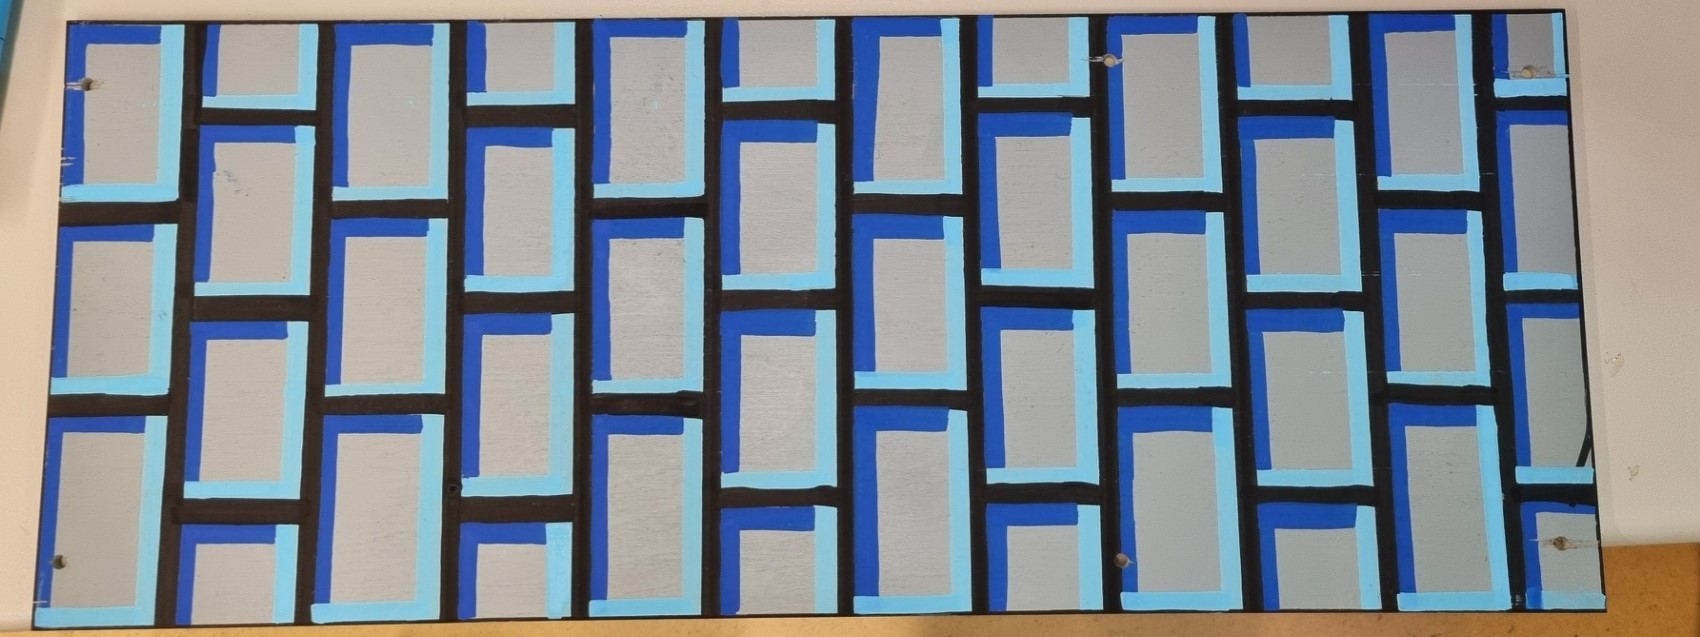
\includegraphics[width=0.5\textwidth]{Abb.16_bemalte_Holzwand.jpg}
		\centering
		\caption{Abb.3}
	\end{figure}	
	\newpage
	\section{Verkleidung der Frontöffnung} 
	Die Verkleidung (Abb.4) für die Öffnung wird mit Kraftkleber an der Holzwand befestigt(Abb.5).
\begin{figure}[htb]
		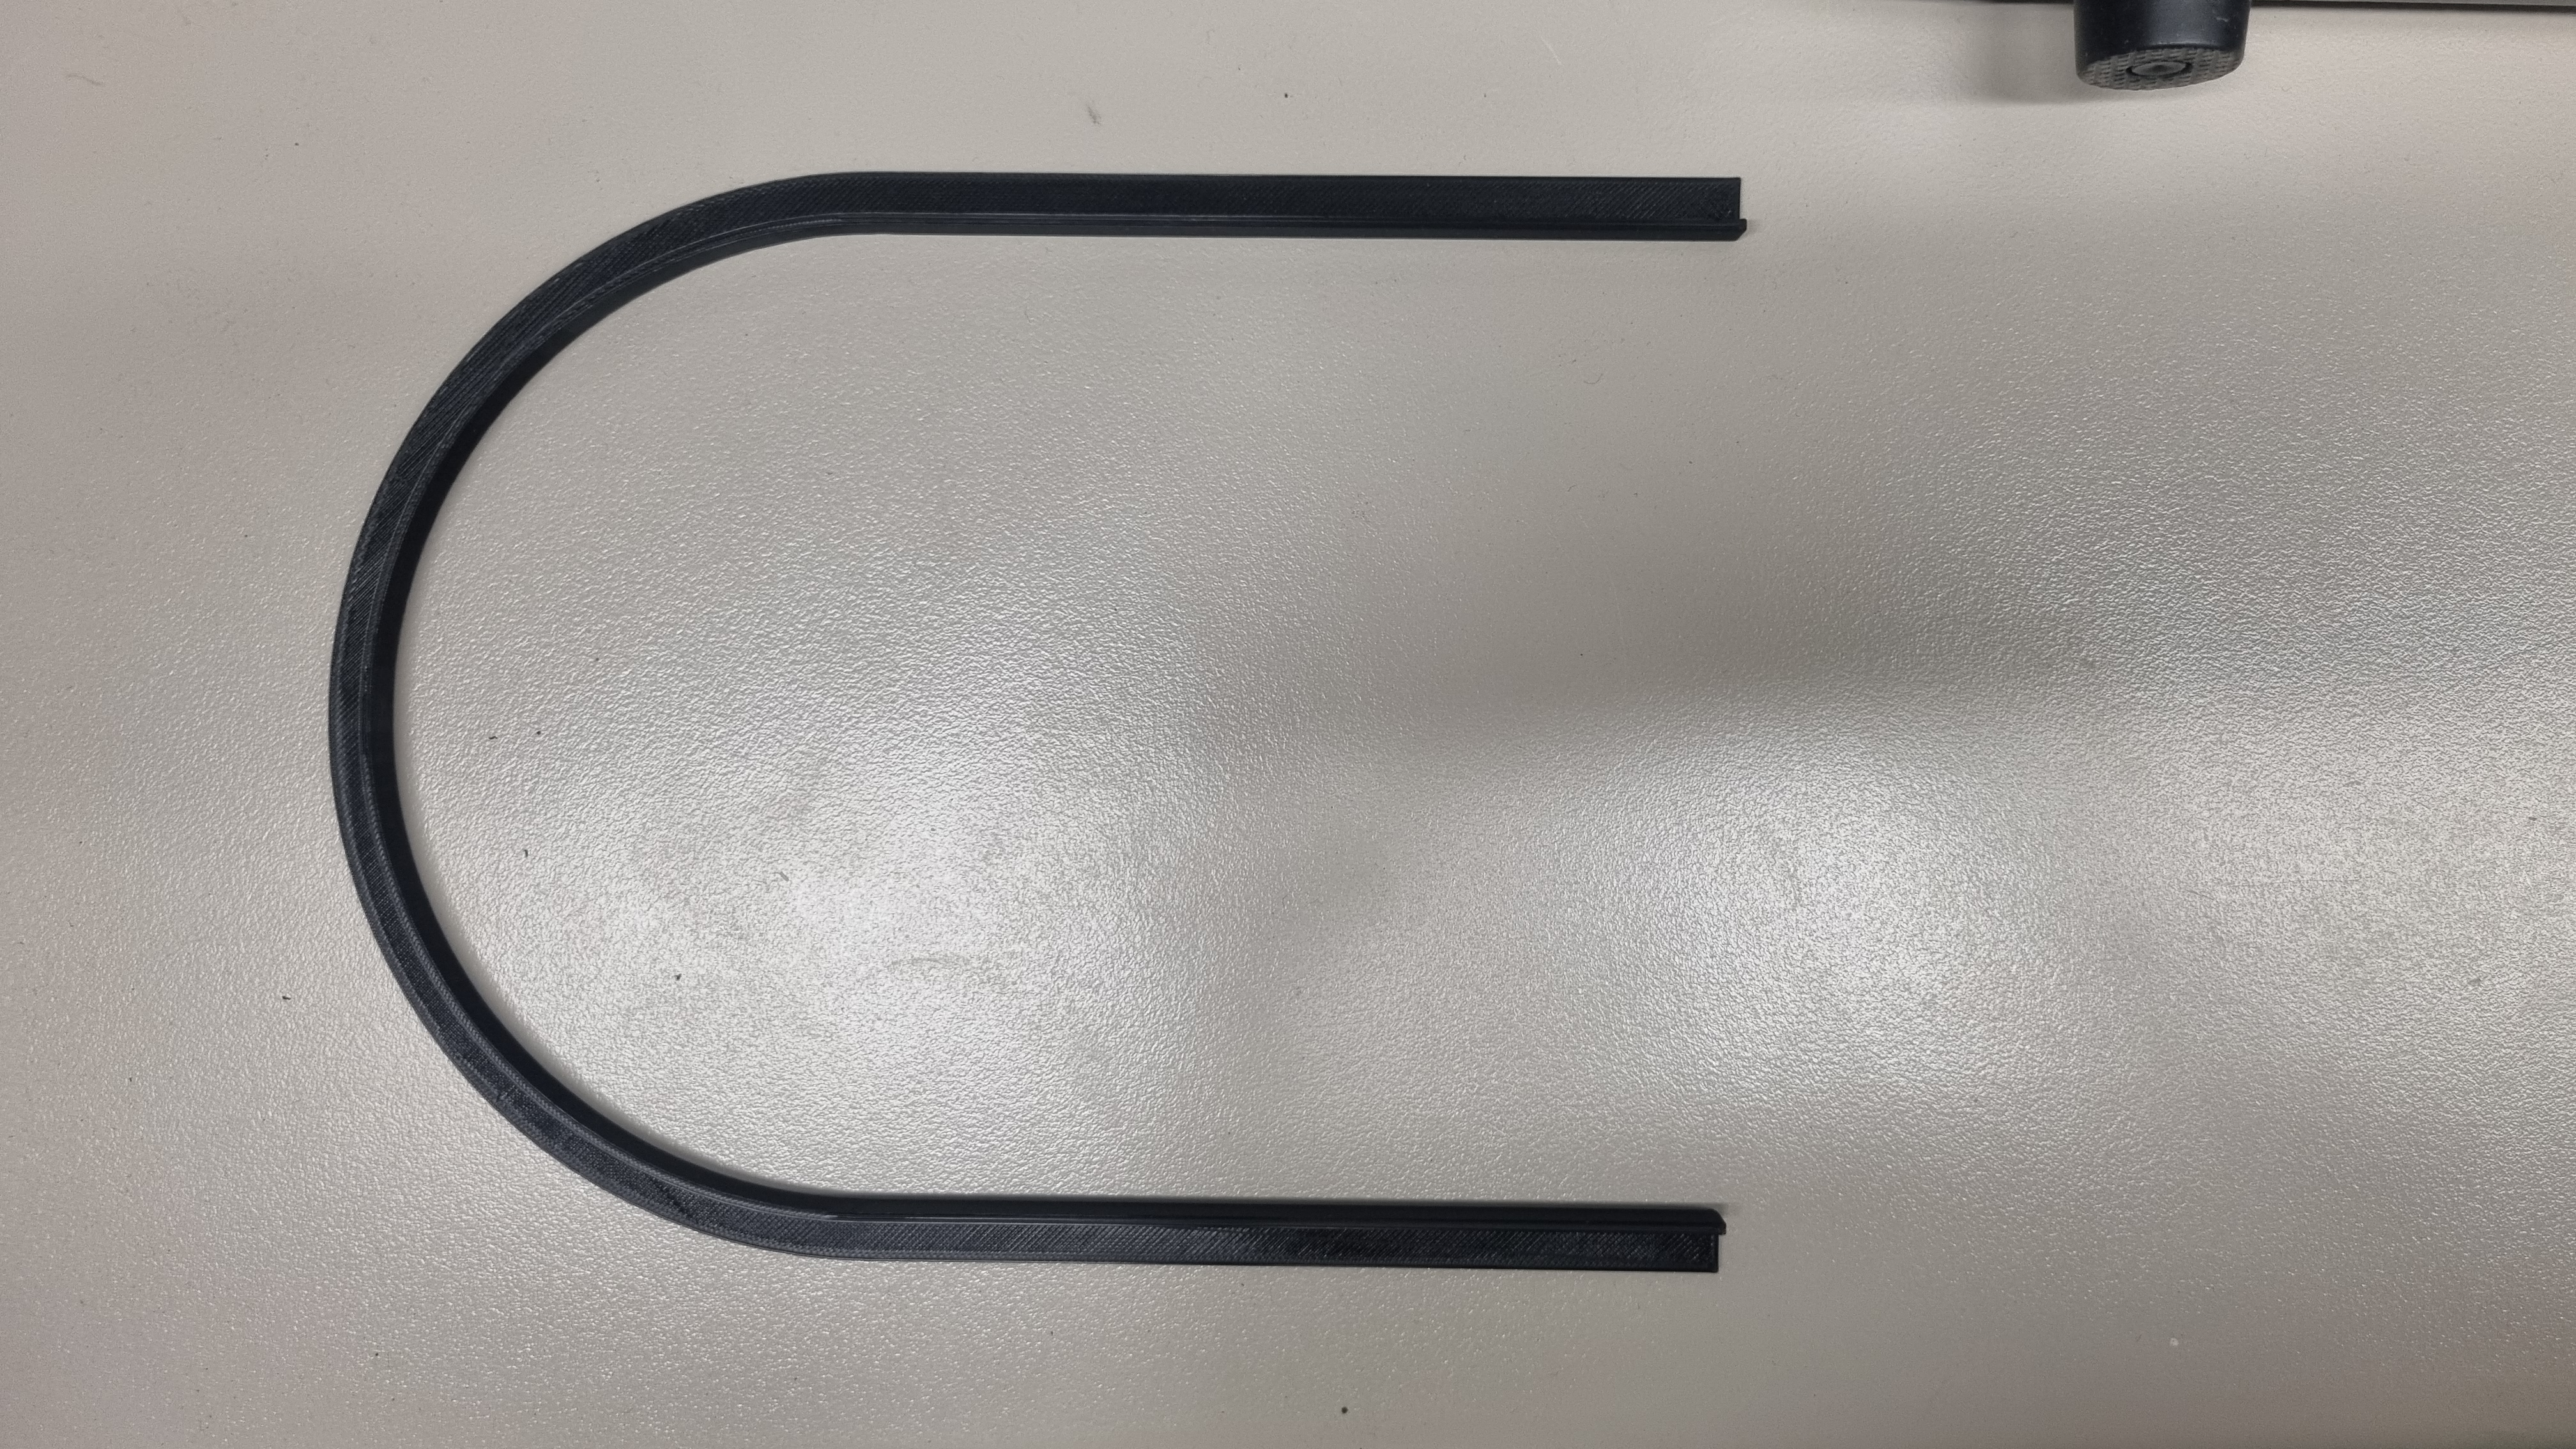
\includegraphics[width=0.5\textwidth]{Abb.4_Verkleidung.jpg}
		\centering
		\caption{Abb.4}
	\end{figure}
	\begin{figure}[htb]
		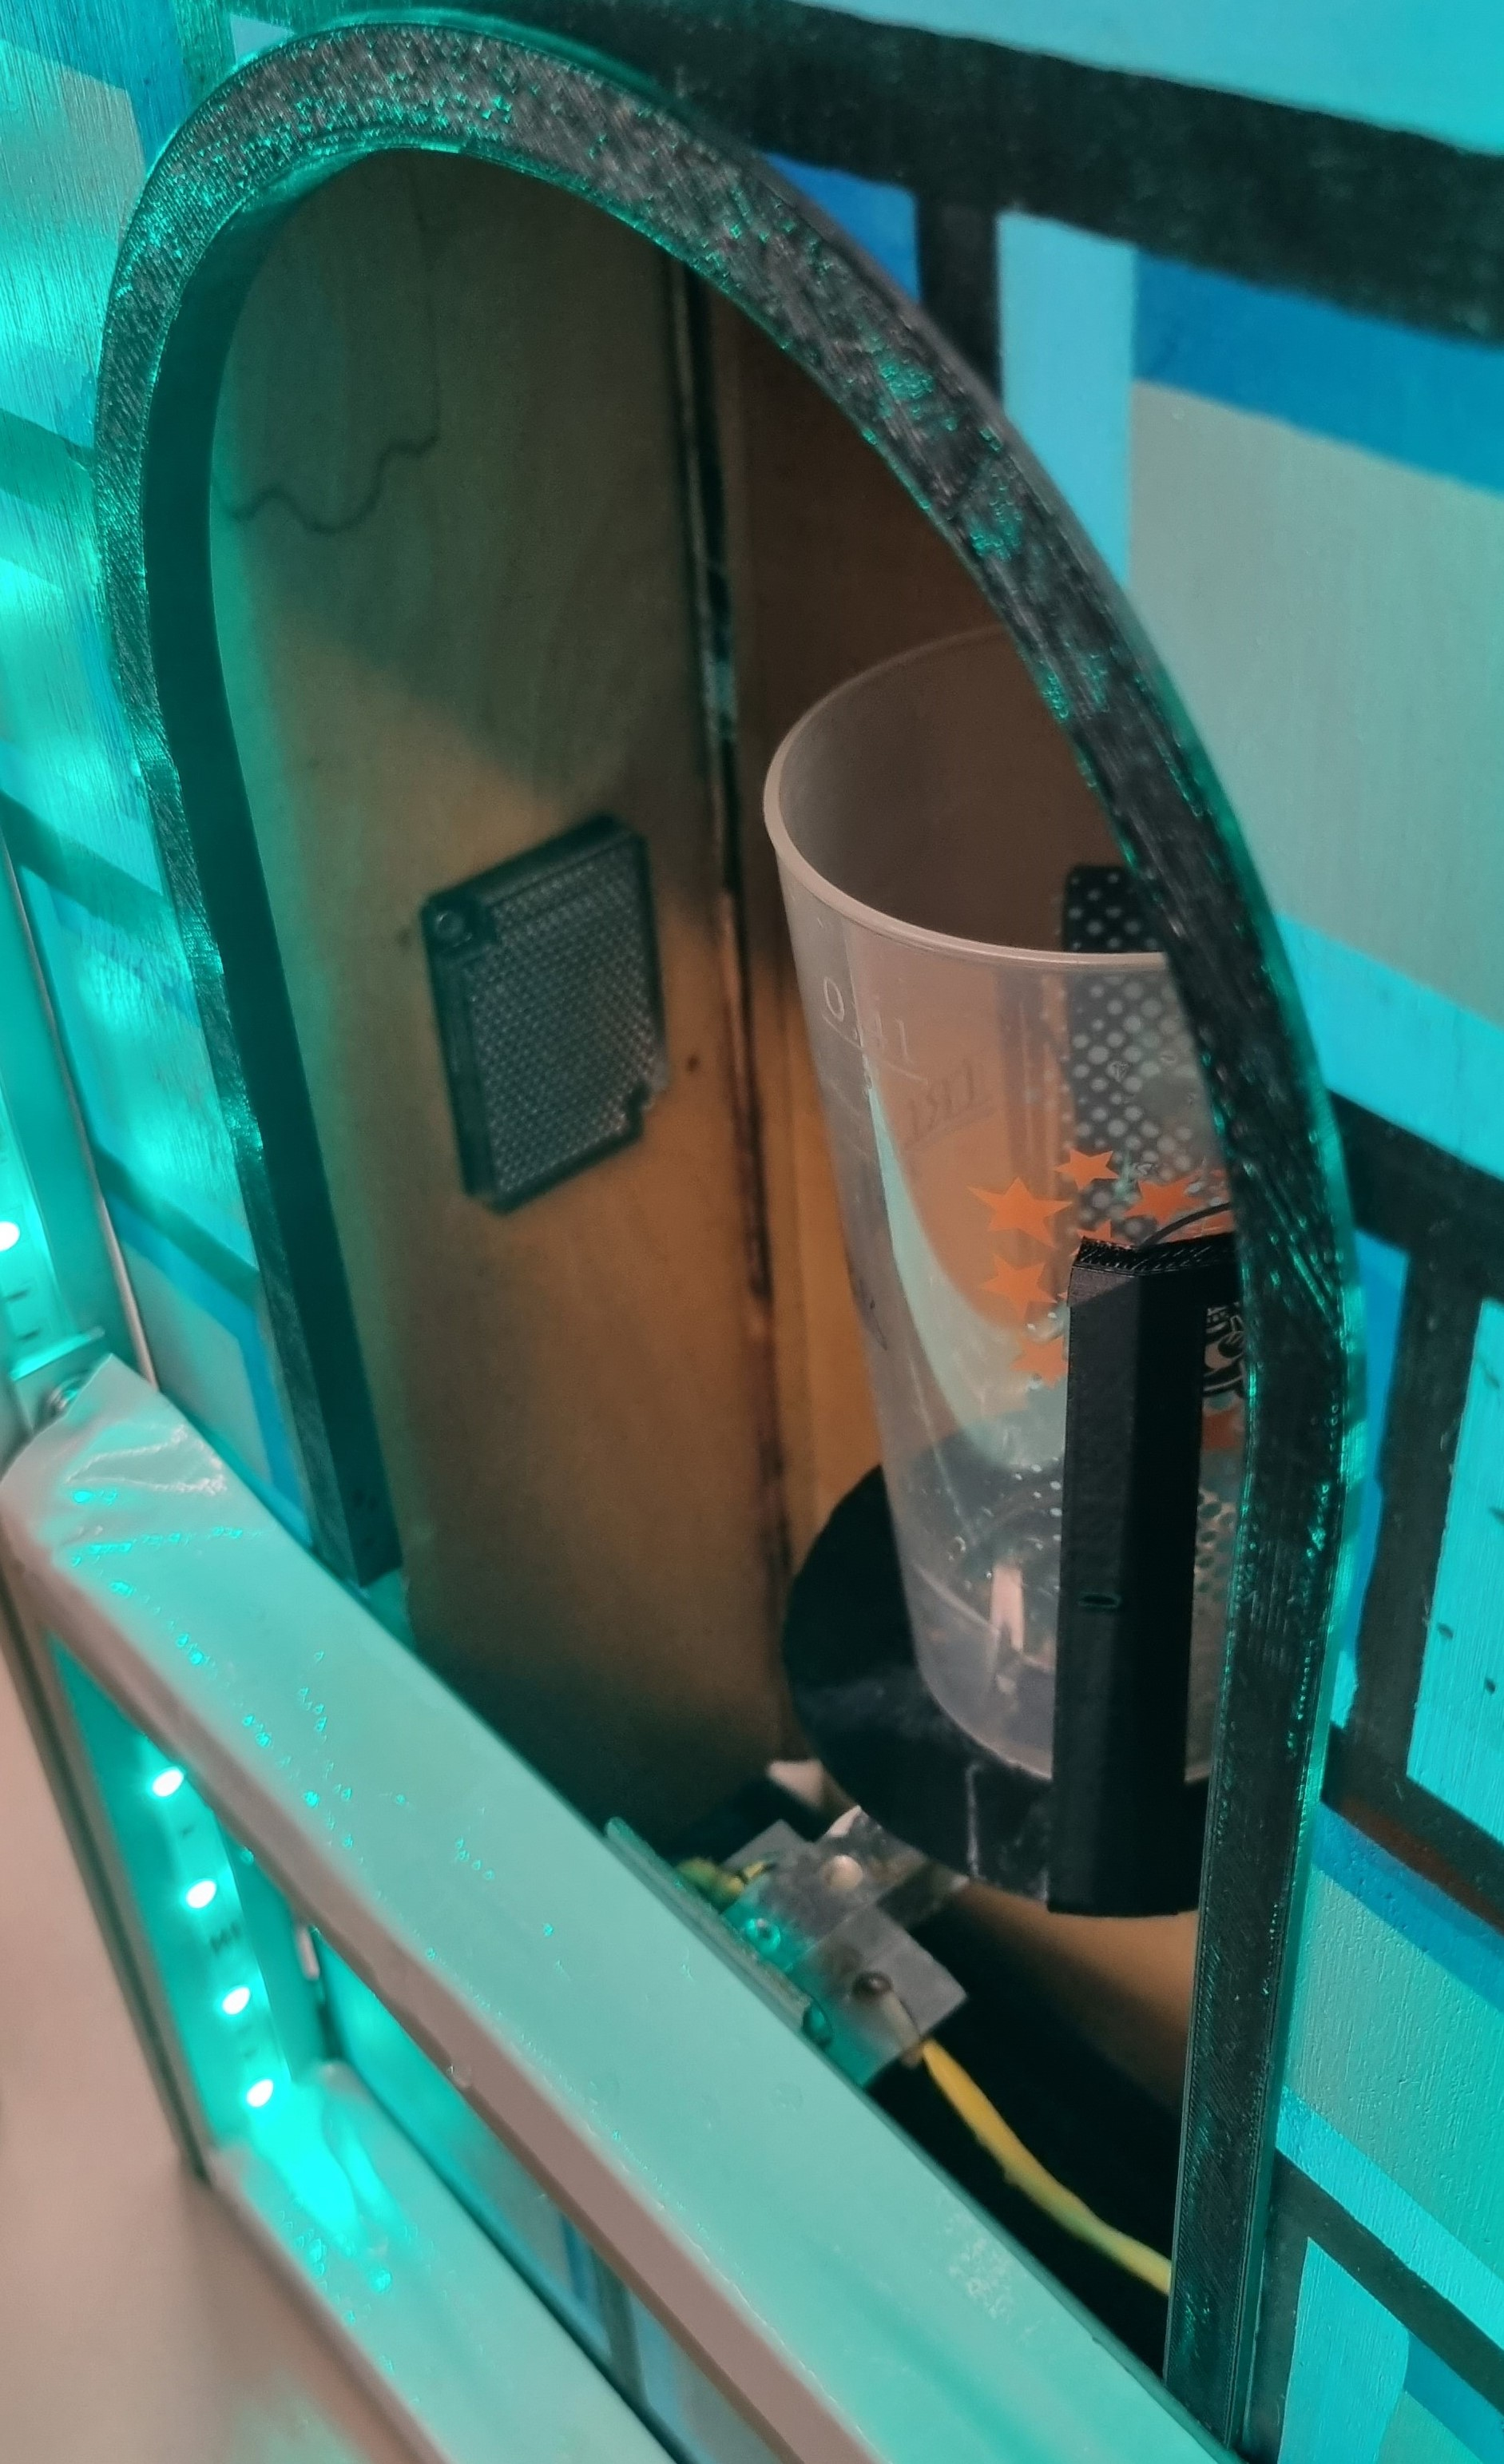
\includegraphics[width=0.5\textwidth]{Abb.5_Verkleidung_befestigt.jpg}
		\centering
		\caption{Abb.5}
	\end{figure}
	\chapter{Komponentenmontage}
	\section{Wägezelle}
	1.\\
	Die Becherhalterung wird an dem Becherständer mittels Kraftkleber montiert.
	\\ \\
	2.\\ 
	Die zusammengesetzte Konstruktion wird mit einer Schraube an die Wägezelle (Äußeres Loch) befestigt.
	
	
	\chapter{Verkabelung}
	
	Die Verkabelung wird mit Hilfe der Stromlaufplänen realisiert(Abb.  ). Dabei werden Kupferkabel mit einer Querschnittsfläche von 0,75 mm² genutzt und an deren Enden, wenn möglich Aderendhülsen genutzt Ansonsten werden Lötverbindungen hergestellt.\\
	Hierbei fangen wir mit der Verkabelung der SPS an, enden mit der Verkabelung der LEDs. Für die LED-Verkabelung wird gemäß Schaltplan (Siehe Abb. LEDs), das Steuer und Versorgungsboard auf Lochraster hergestellt.
	\begin{figure}[htb]
		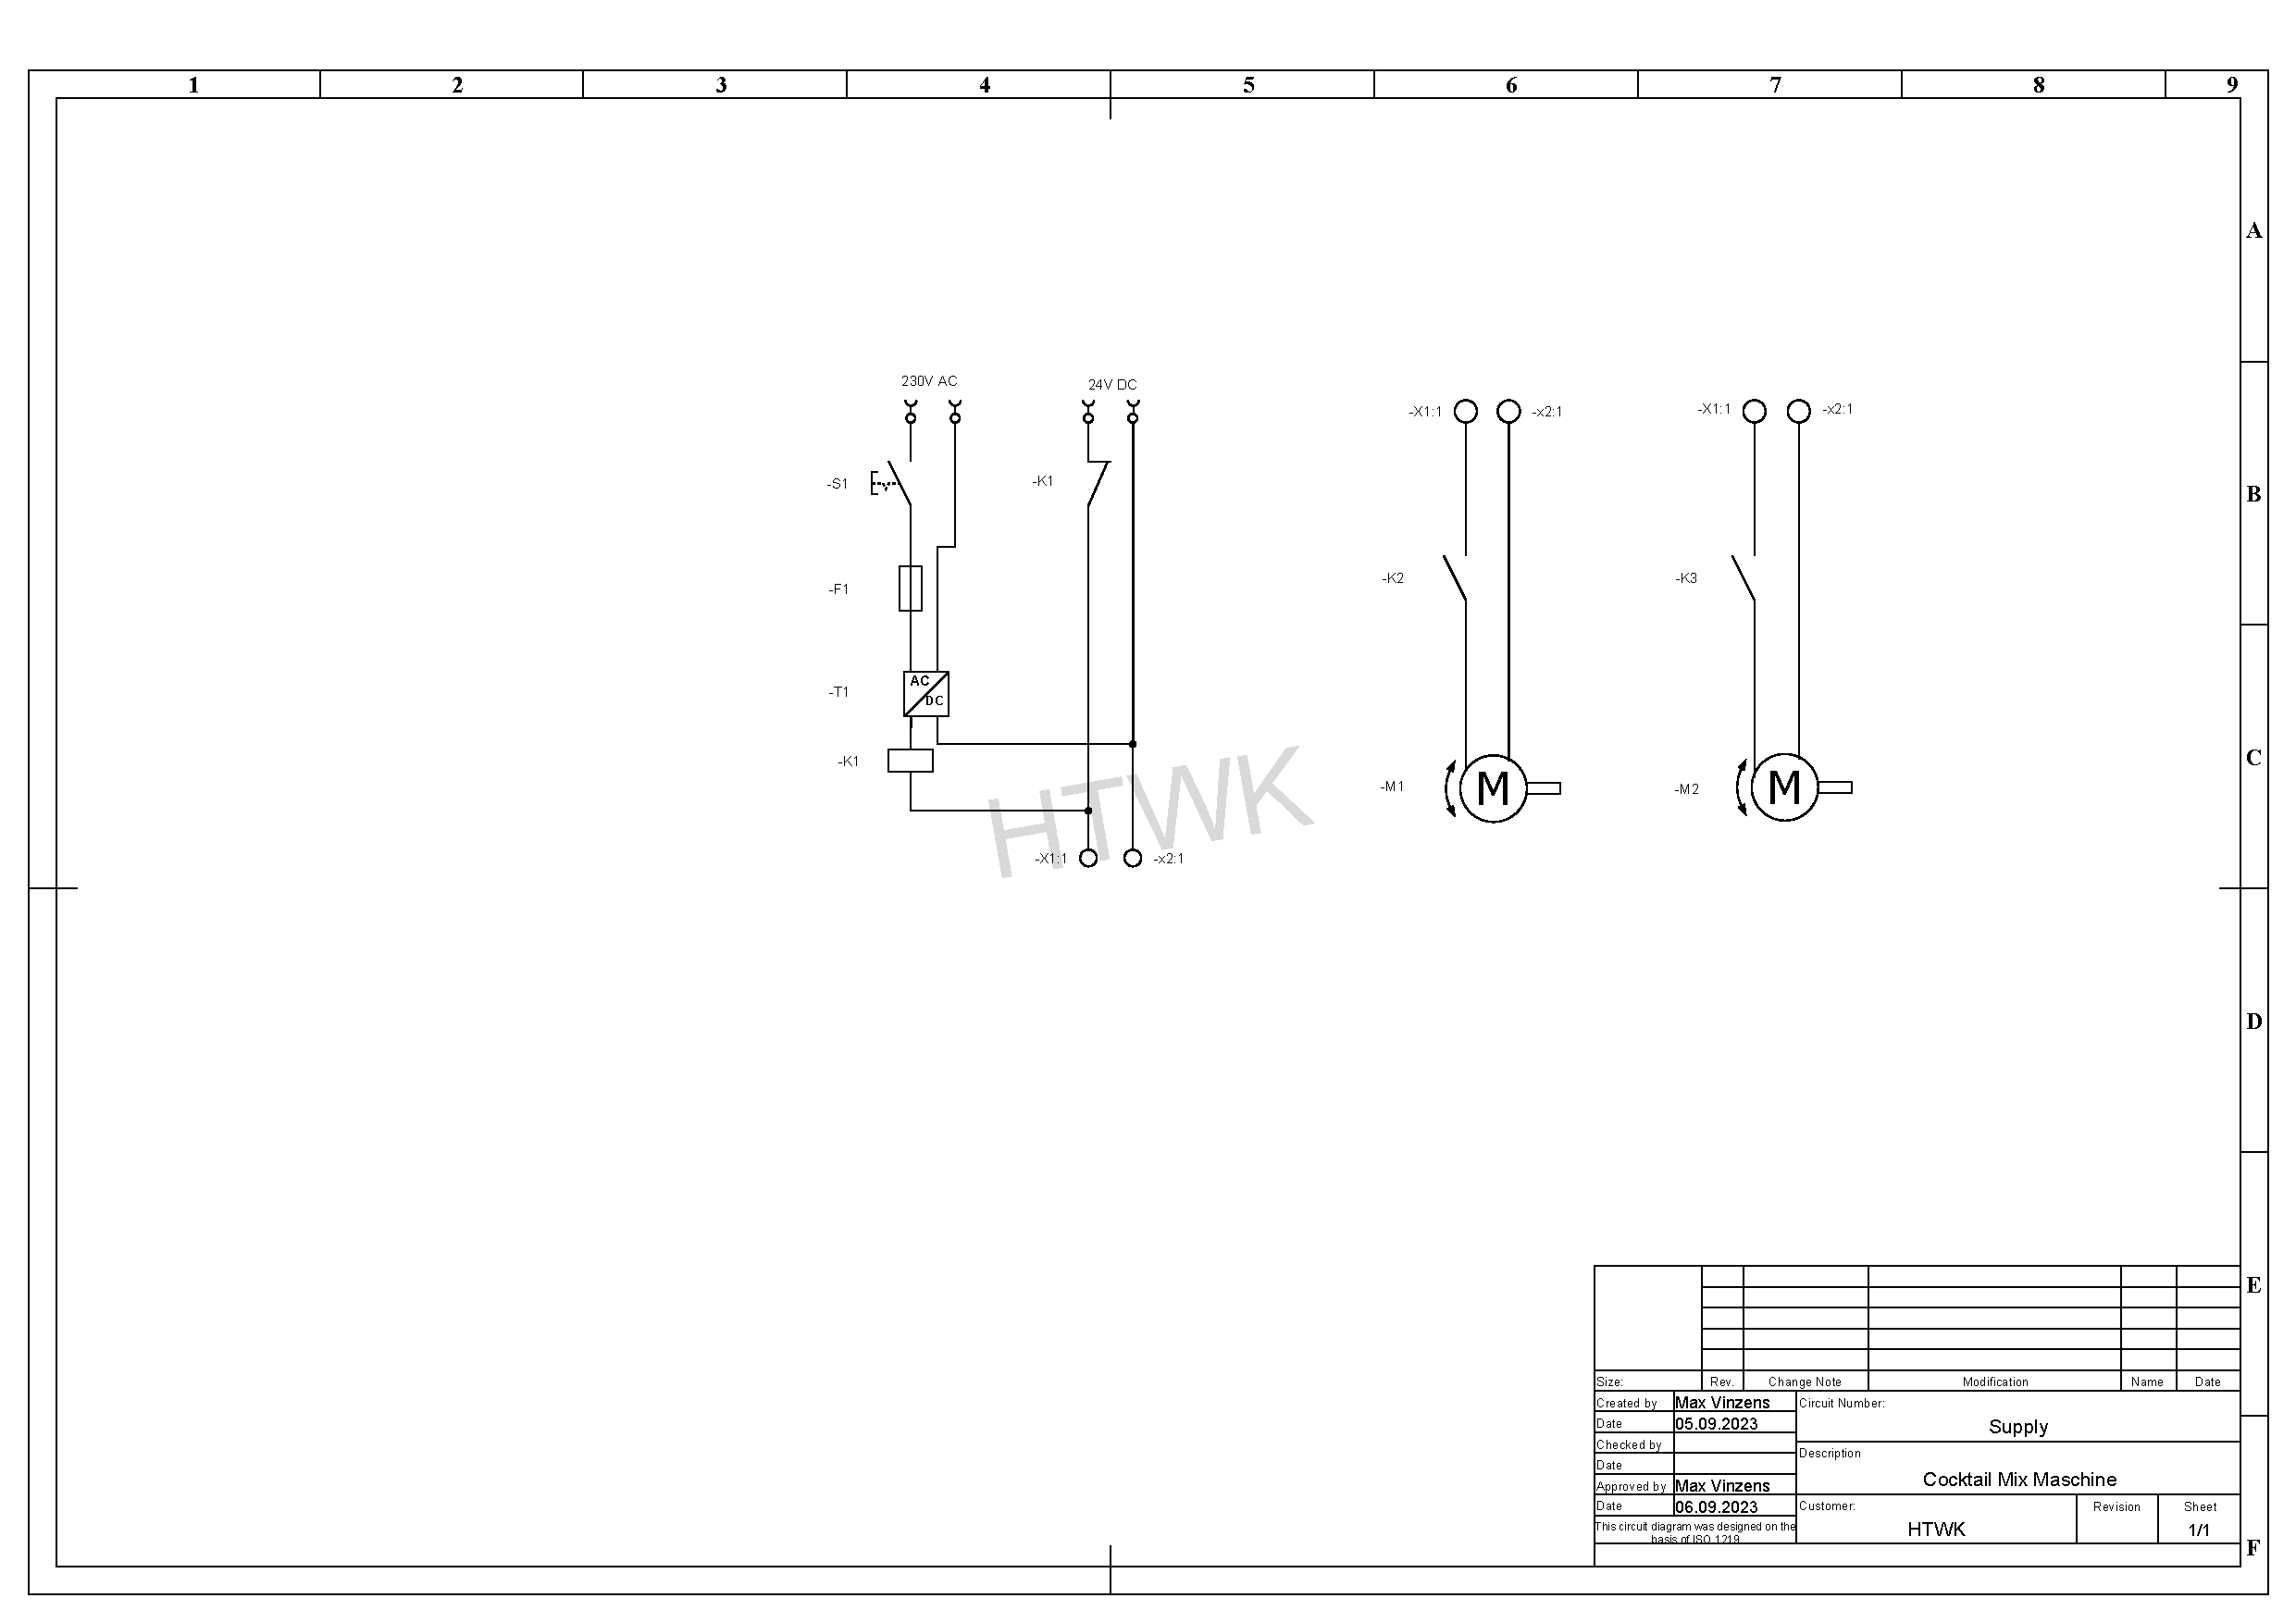
\includegraphics[width=1\textwidth]{Supply (V2) .pdf}
		\centering
		\caption{Stromversorgung und Motoren}
	\end{figure}
	\begin{figure}[htb]
	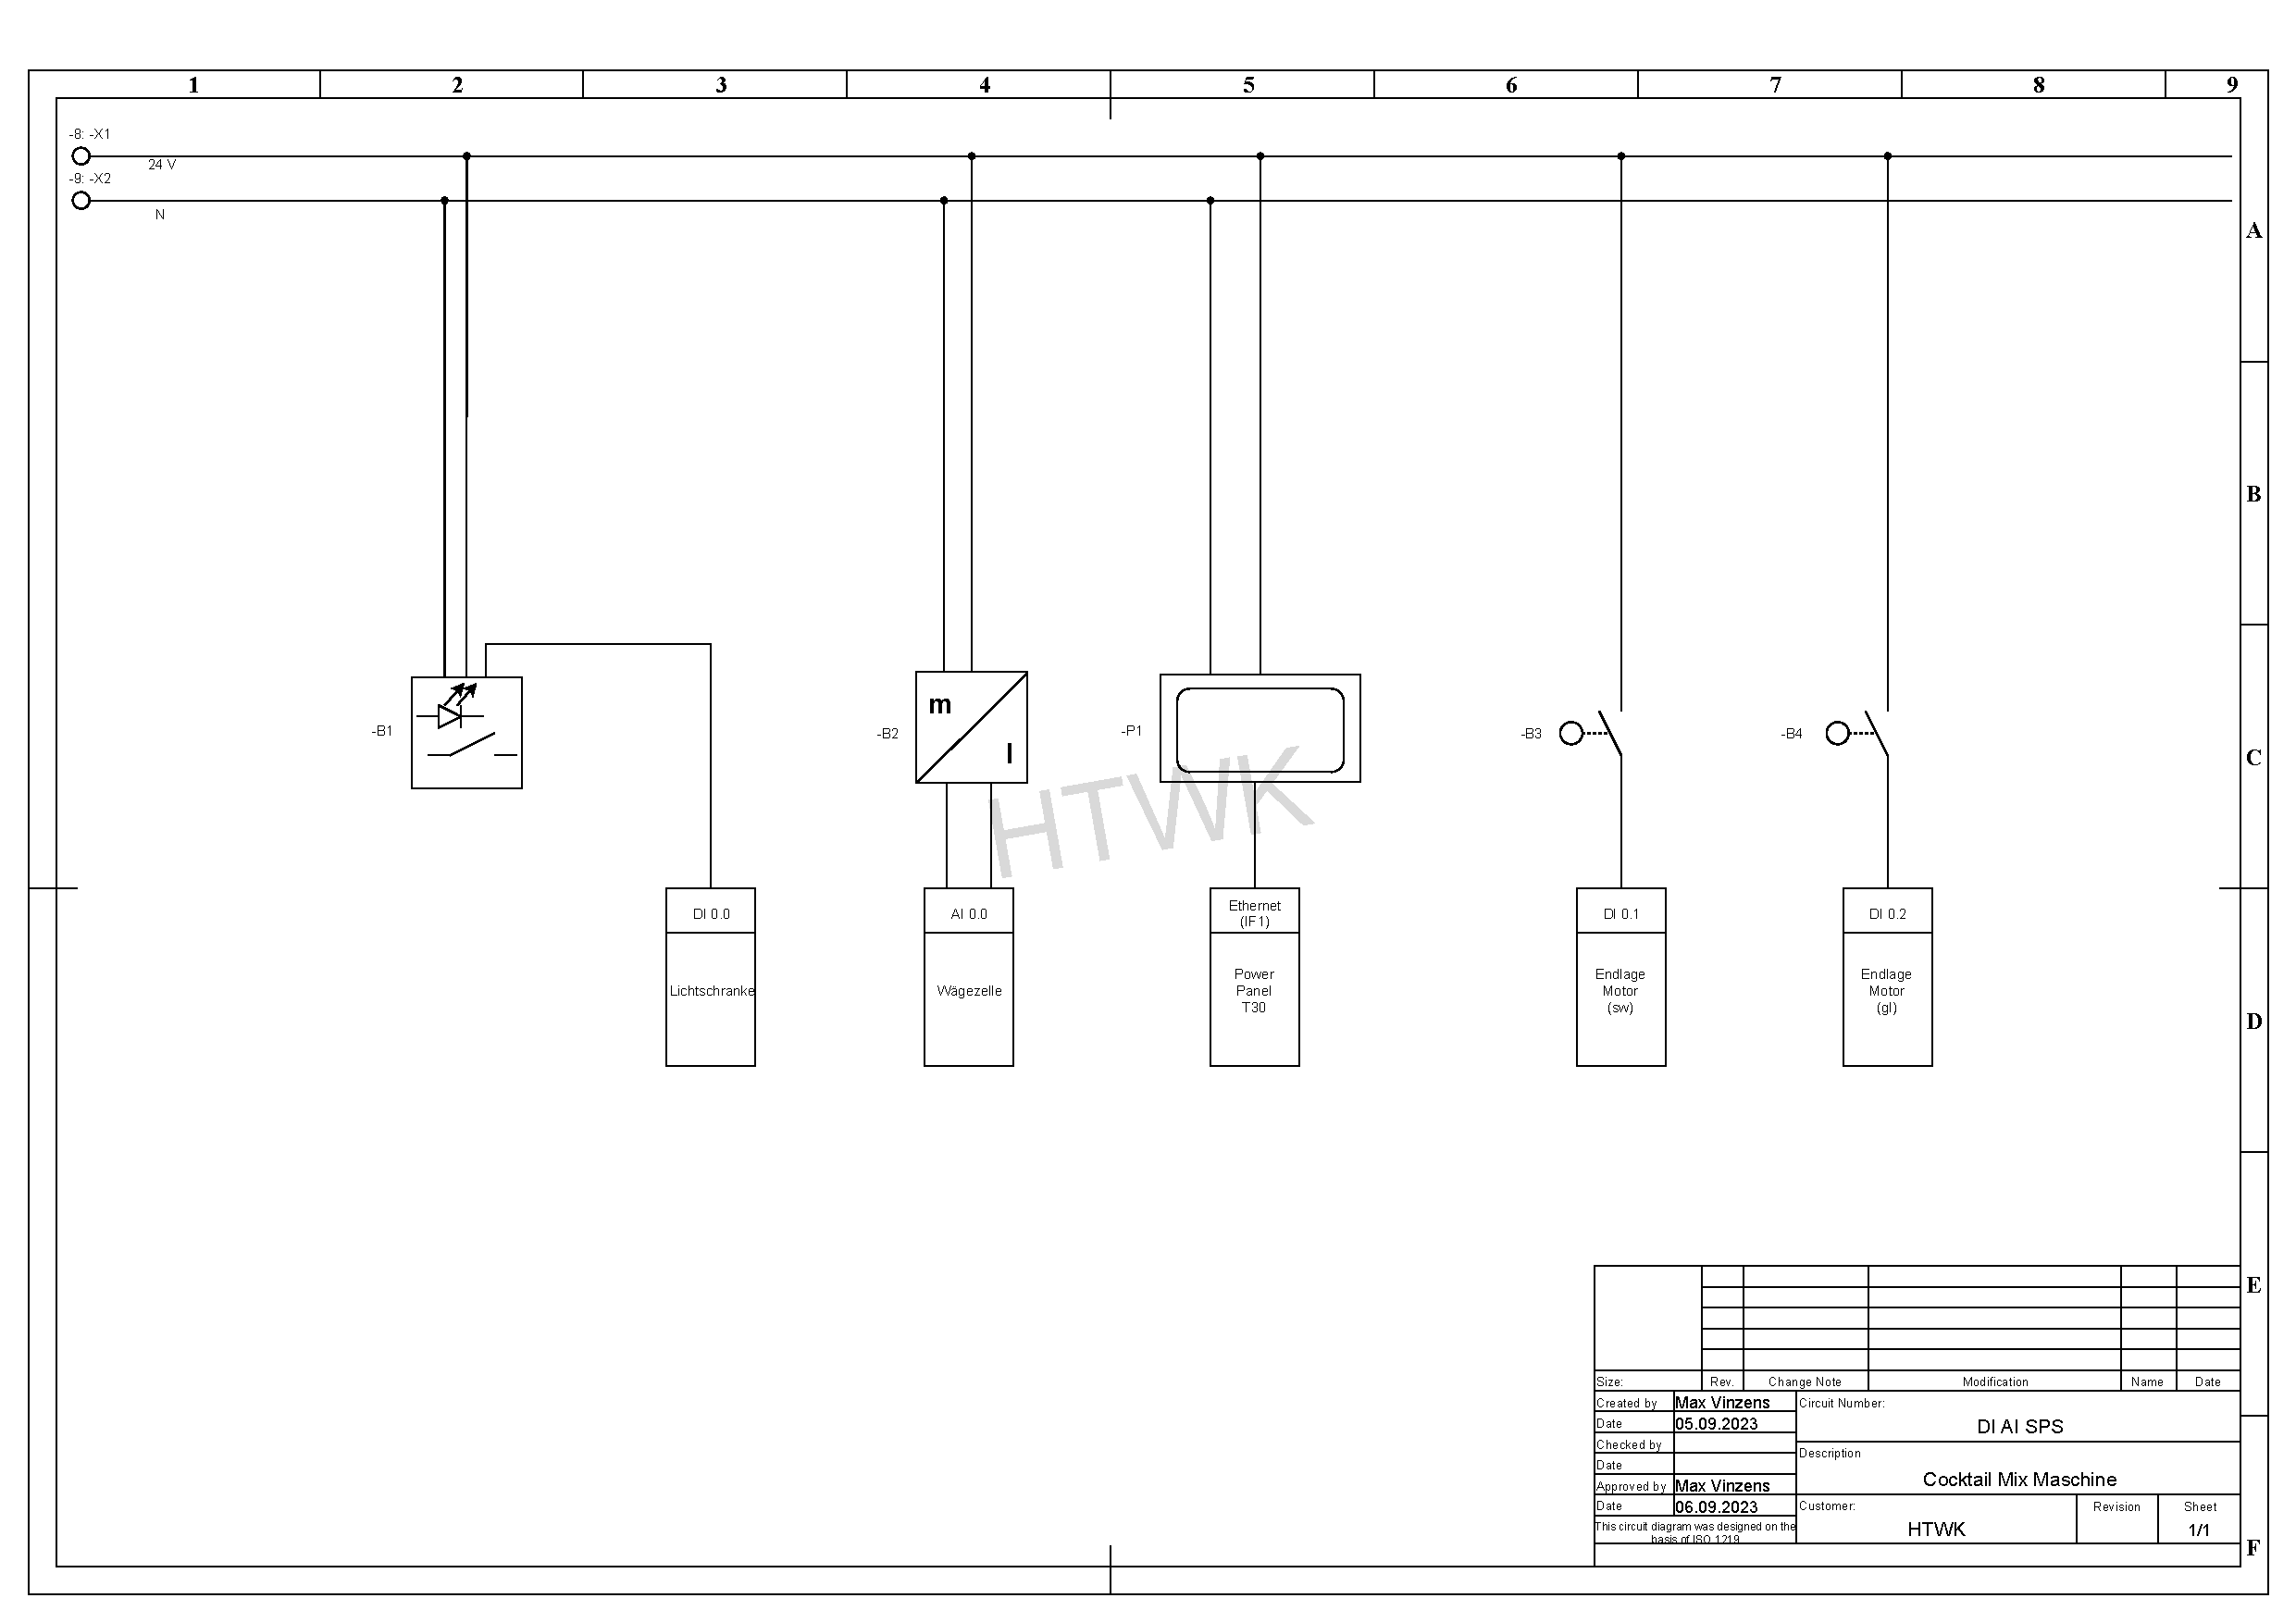
\includegraphics[width=1\textwidth]{DI AI (V2).pdf}
	\centering
	\caption{Eingänge}
	\end{figure}
	\begin{figure}[htb]
		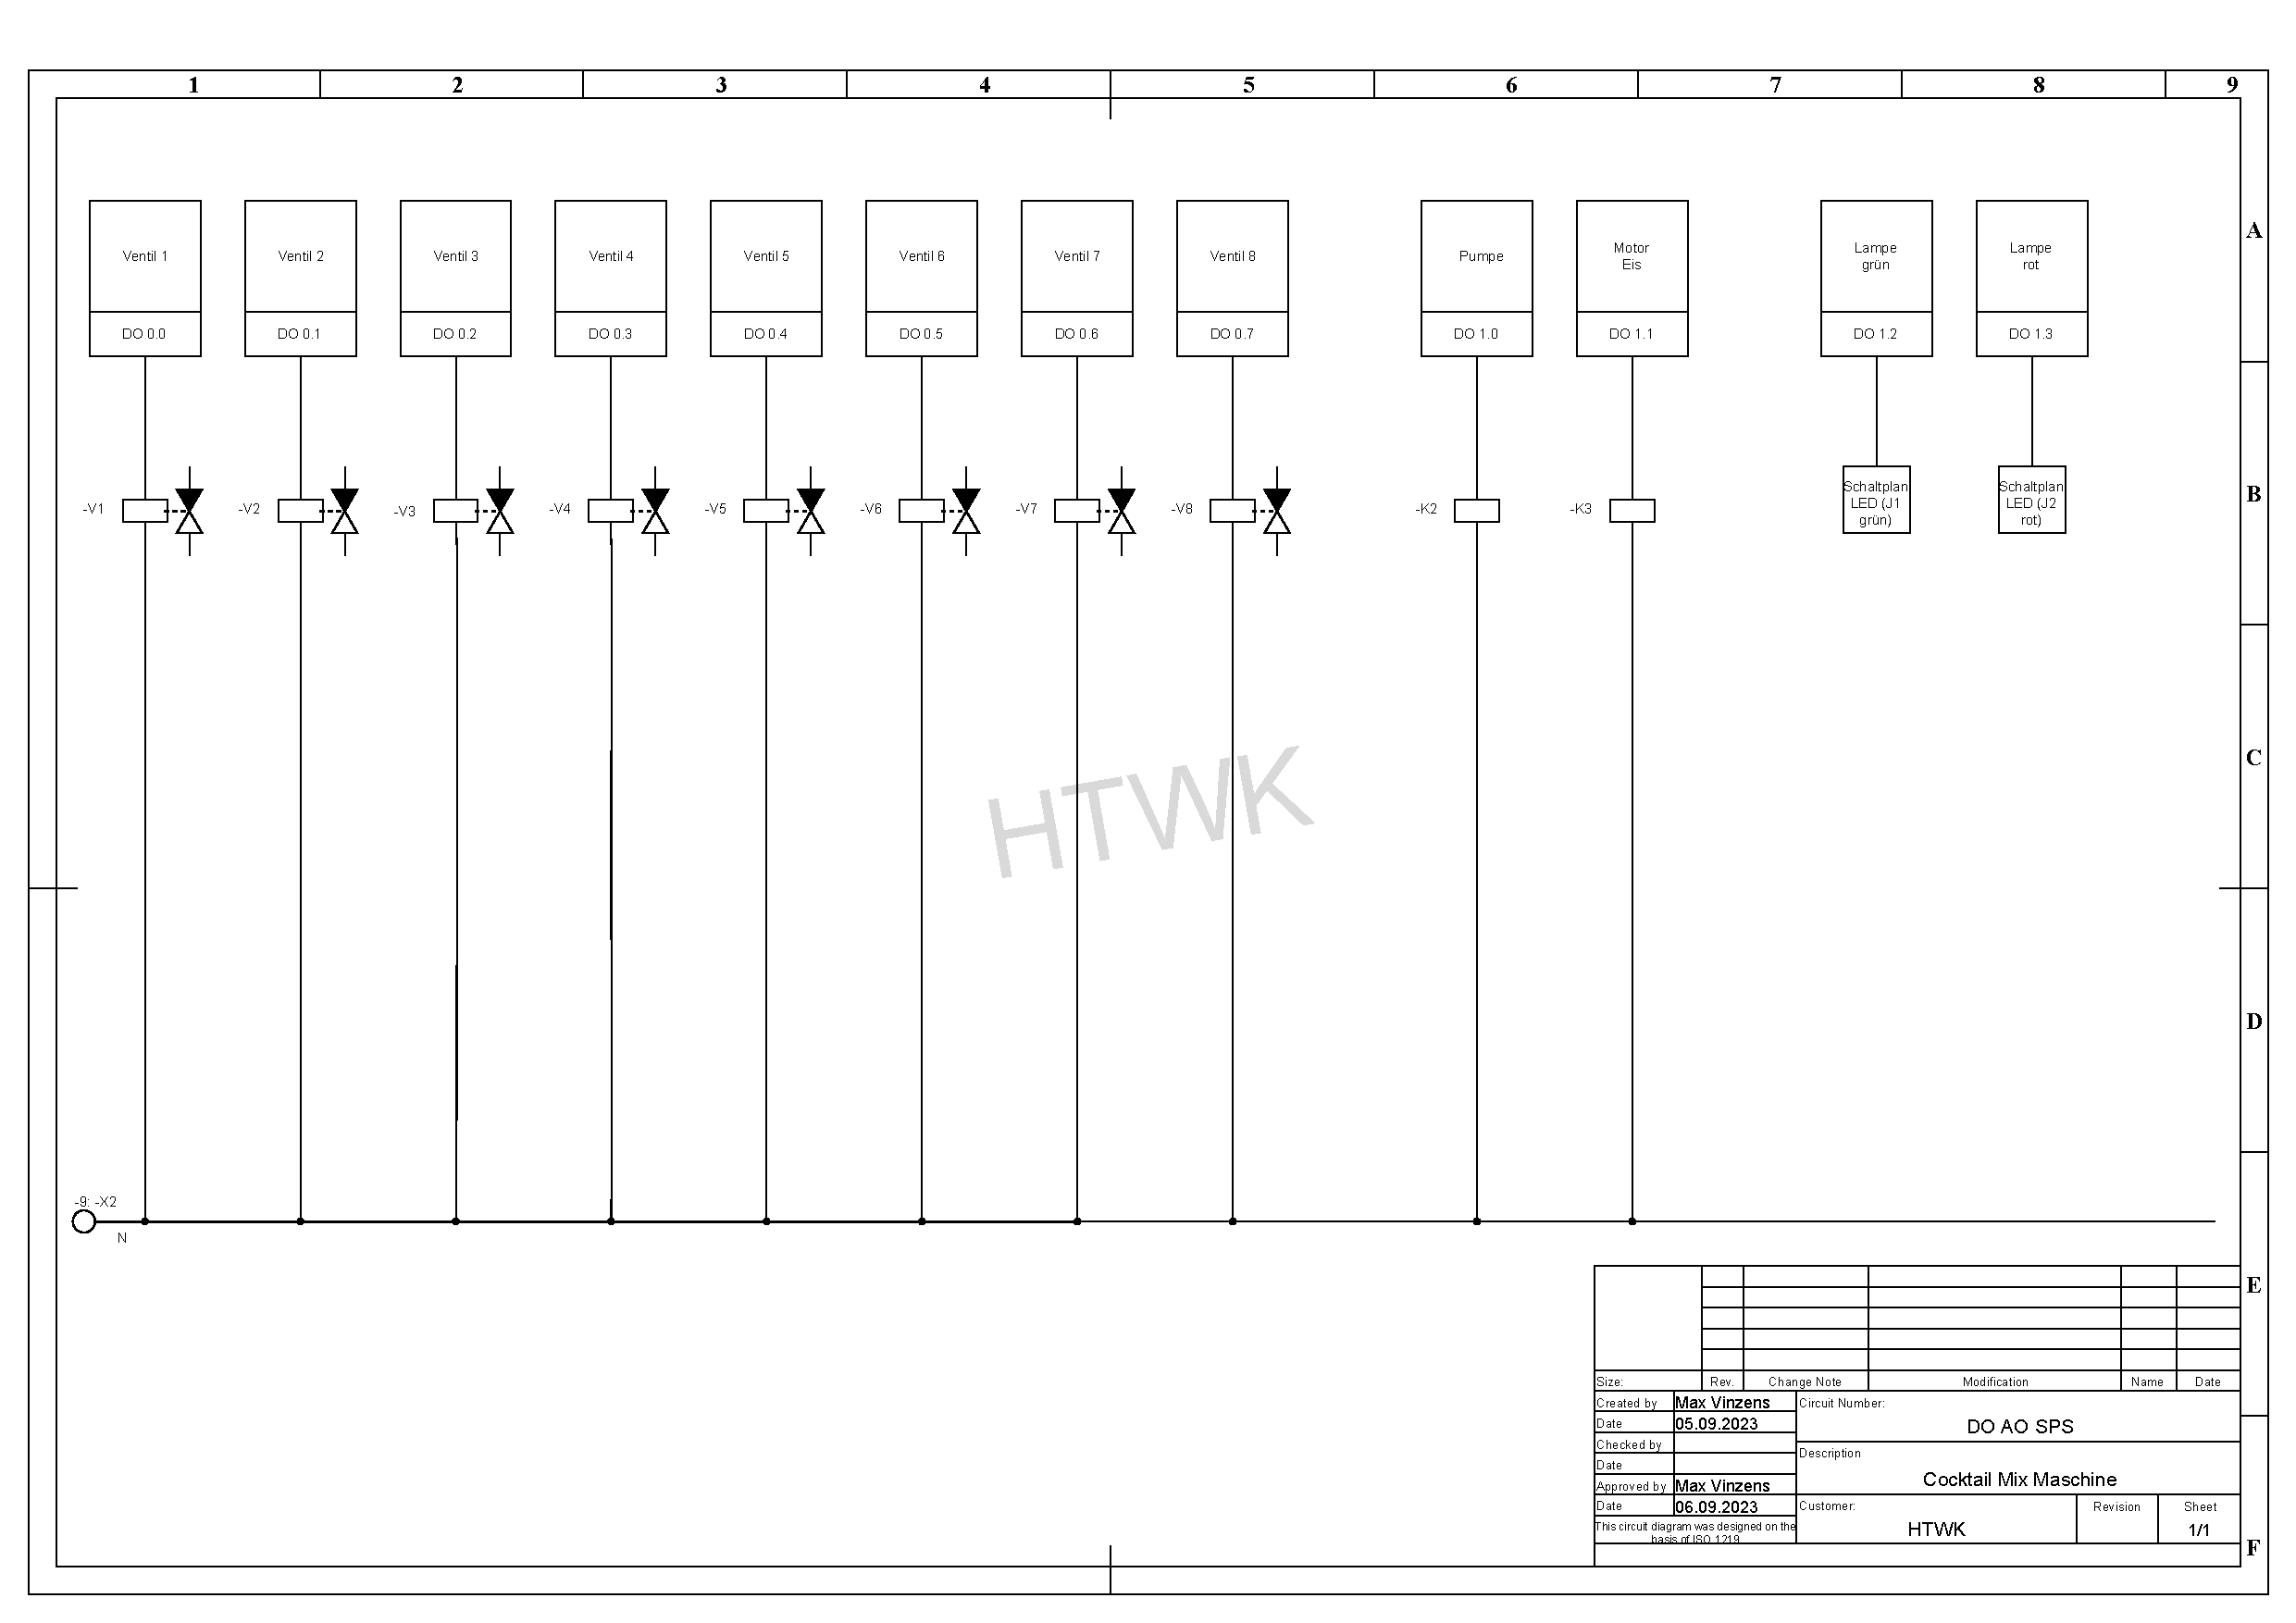
\includegraphics[width=1\textwidth]{DO AO SPS (V2).pdf}
		\centering
		\caption{Ausgänge}
	\end{figure}
	\begin{figure}[htb]
		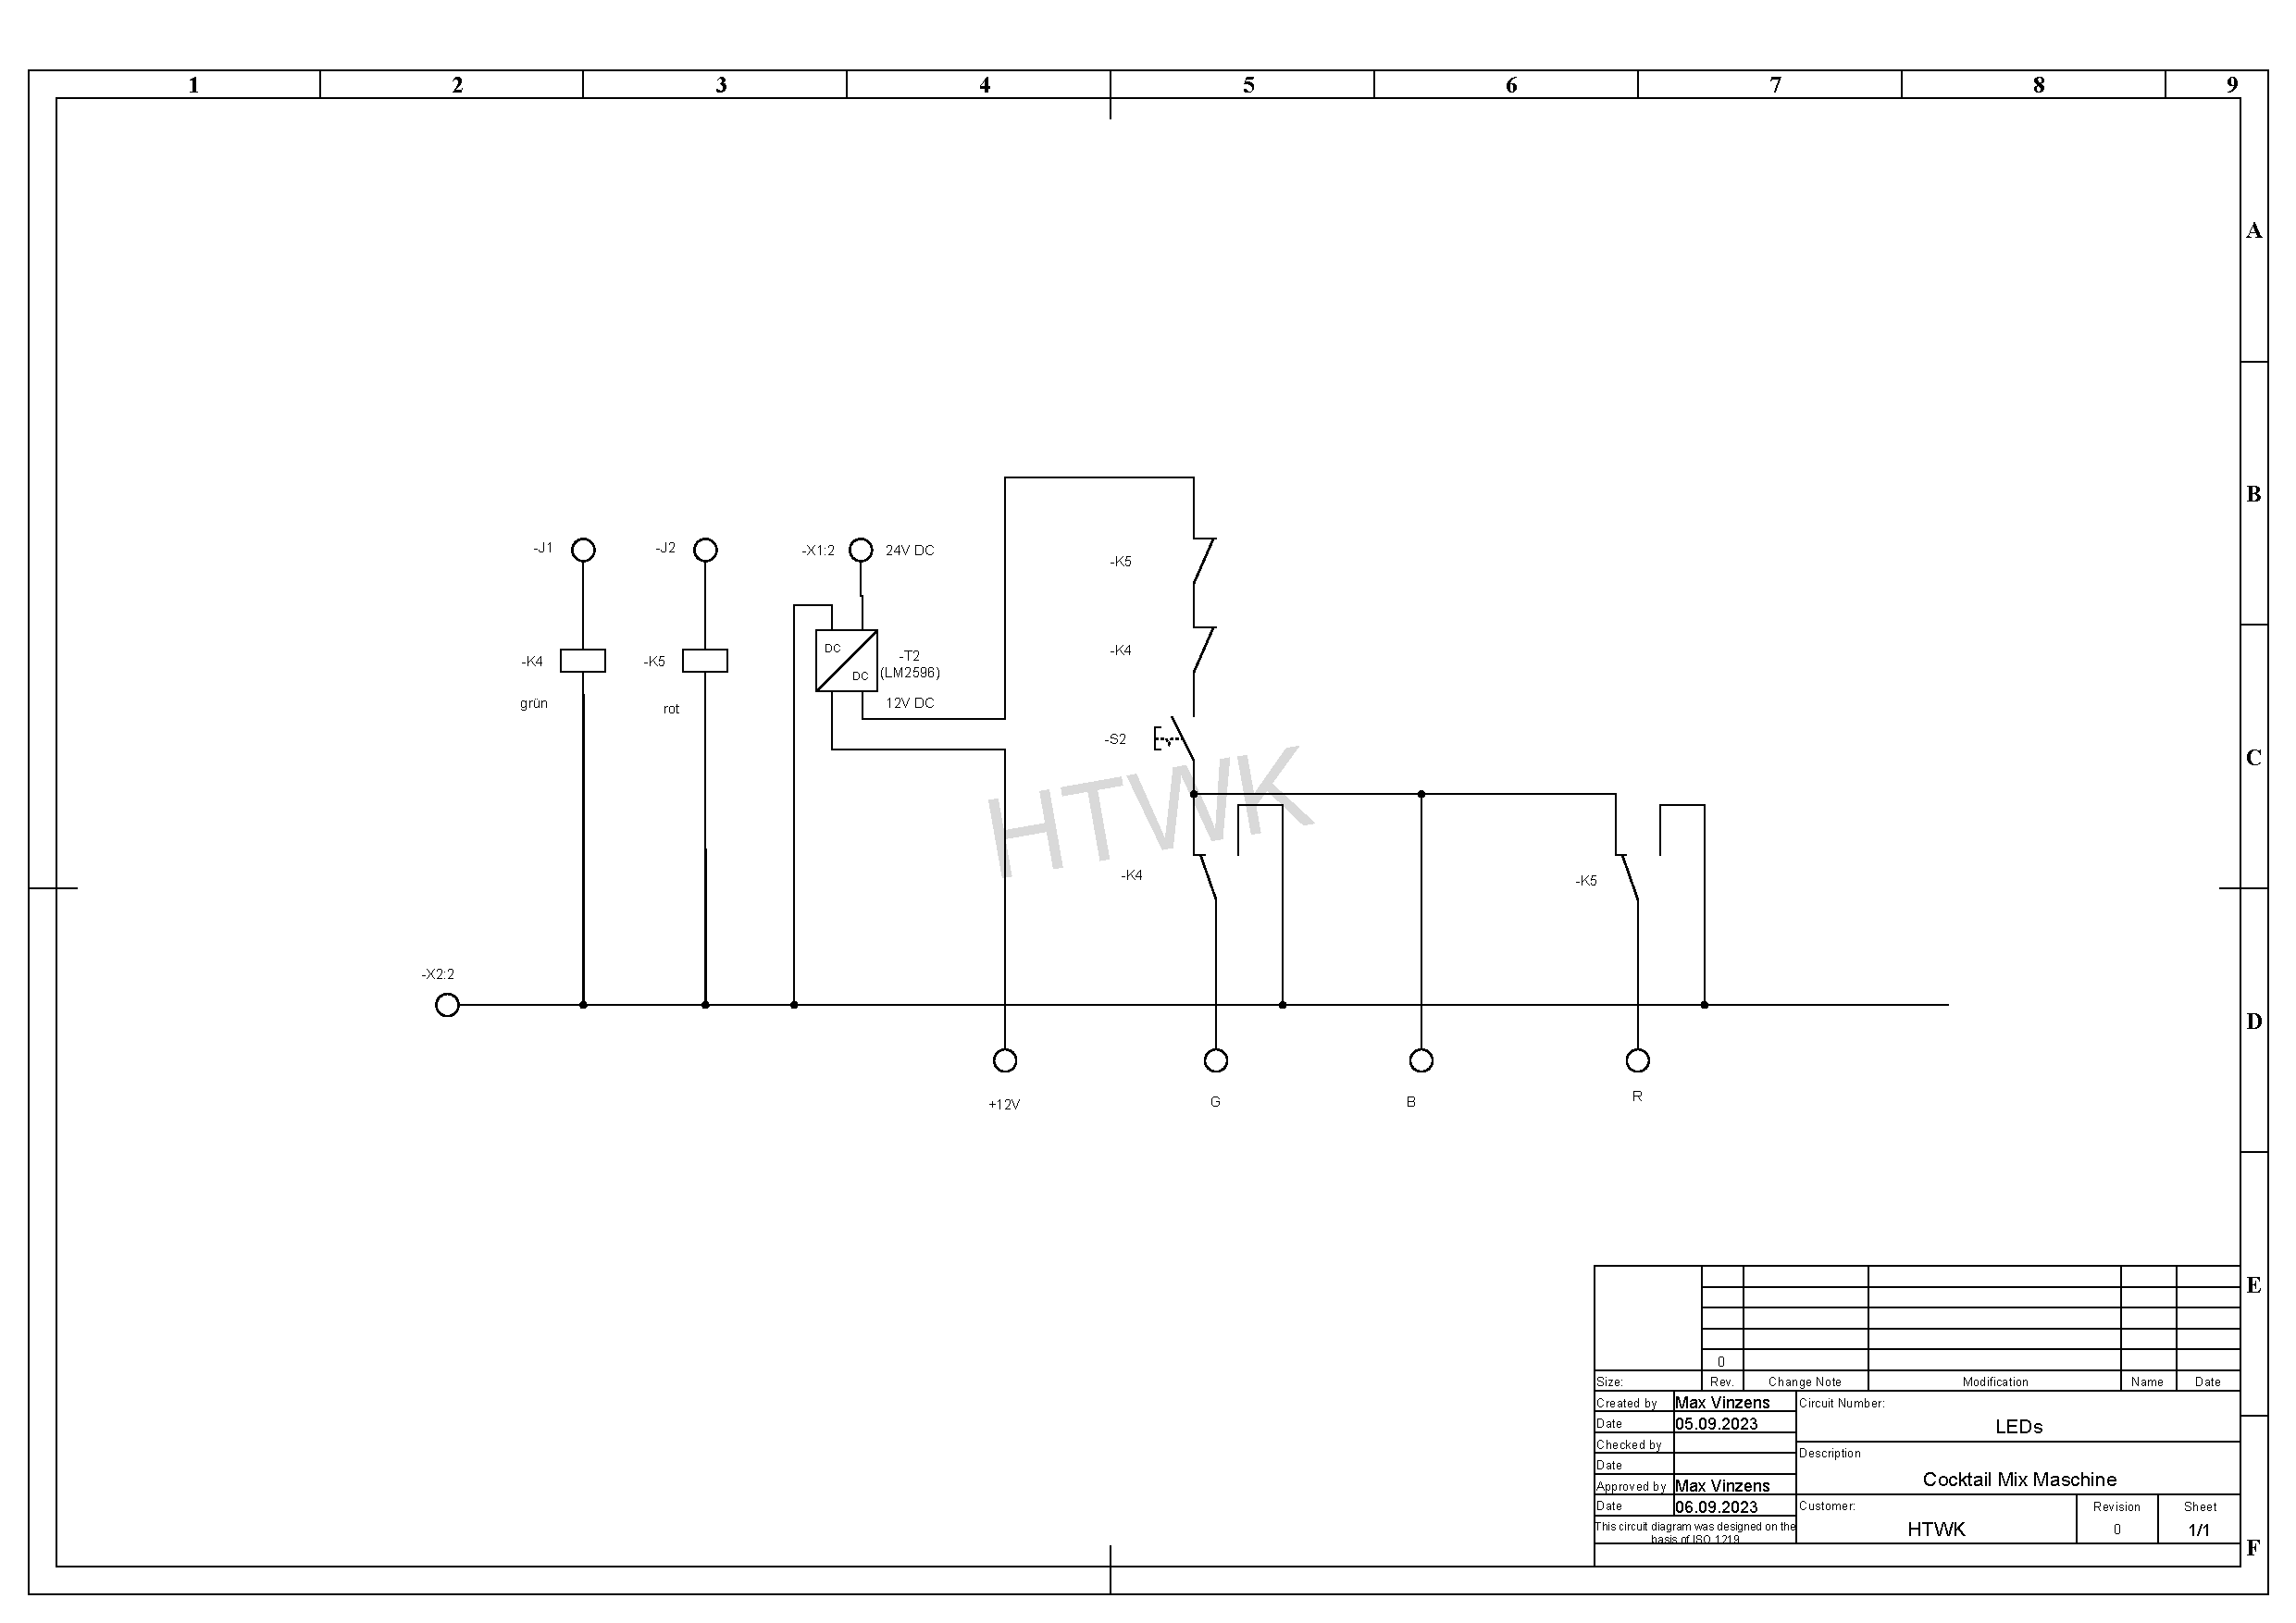
\includegraphics[width=1\textwidth]{LEDs (V2).pdf}
		\centering
		\caption{Leds}
	\end{figure}
	
	

	\chapter{Verschlauchung}
	1.
	
	\begin{figure}[htb]
		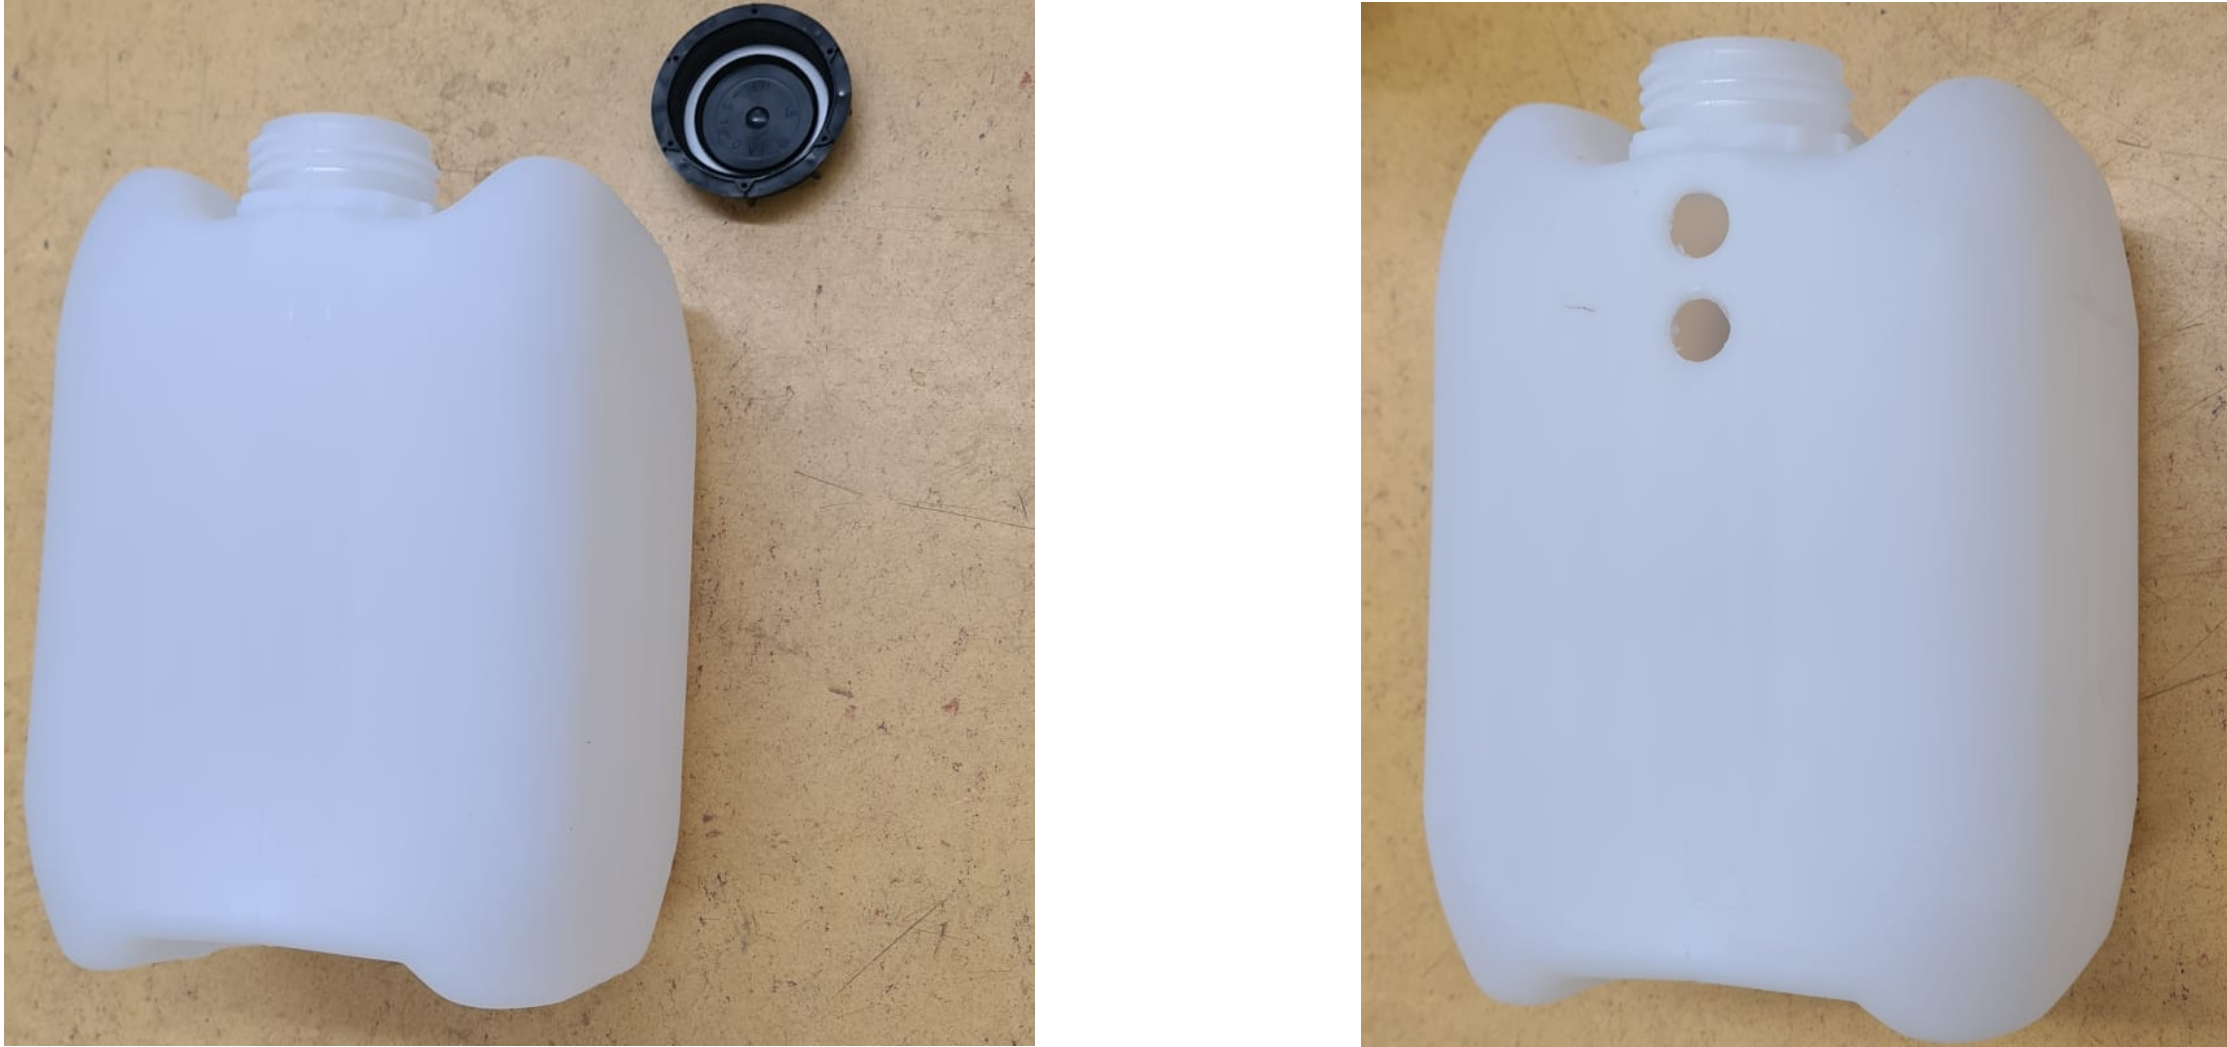
\includegraphics[width=1\textwidth]{zu 1.}
		\centering
		\caption{Am HD-PE Leerkanister bei einer Flachen Seite zwei M16 Löcher Bohren}
	\end{figure}
	
	2.
	
	\begin{figure}[htb]
		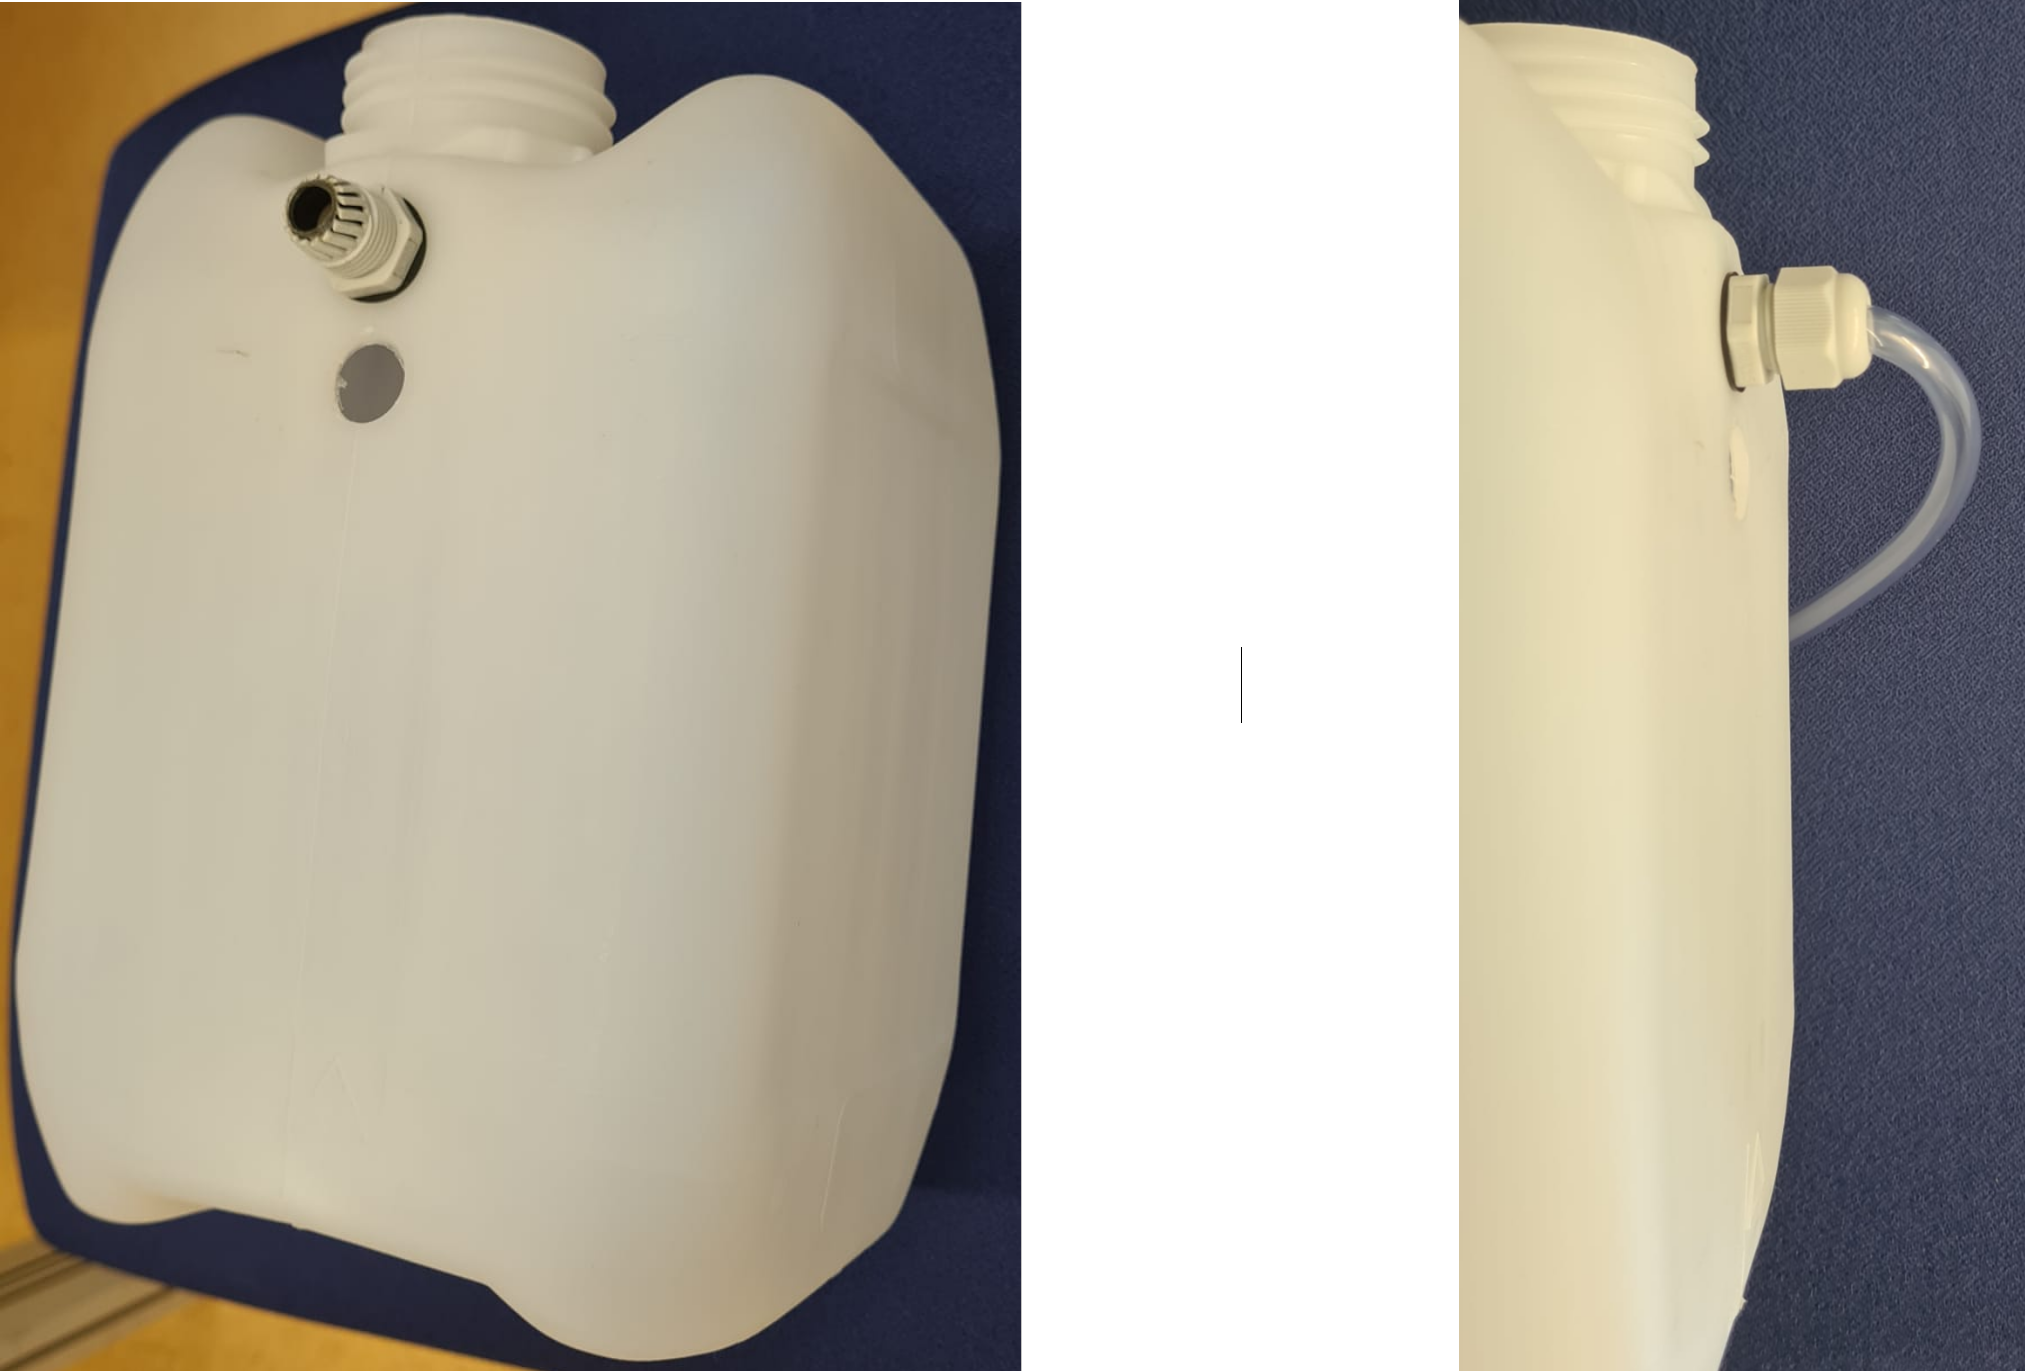
\includegraphics[width=0.8\textwidth]{zu2.}
		\centering
		\caption{Am HD-PE Leerkanister zwei Verschraubungen anbringen. Danach Schlauch befestigen.}
	\end{figure}
	\newpage
	
	3.
	
	\begin{figure}[htb]
		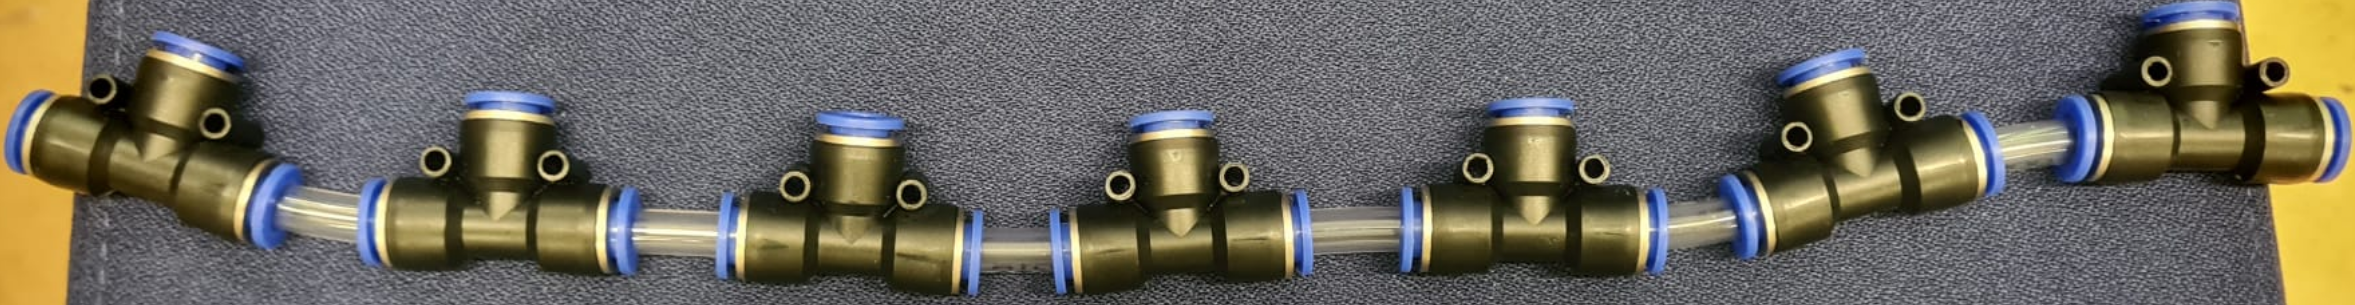
\includegraphics[width=1\textwidth]{zu3.}
		\centering
		\caption{Die T Stücke untereinander verbinden.}
	\end{figure}
	
	4.
	
	\begin{figure}[htb]
		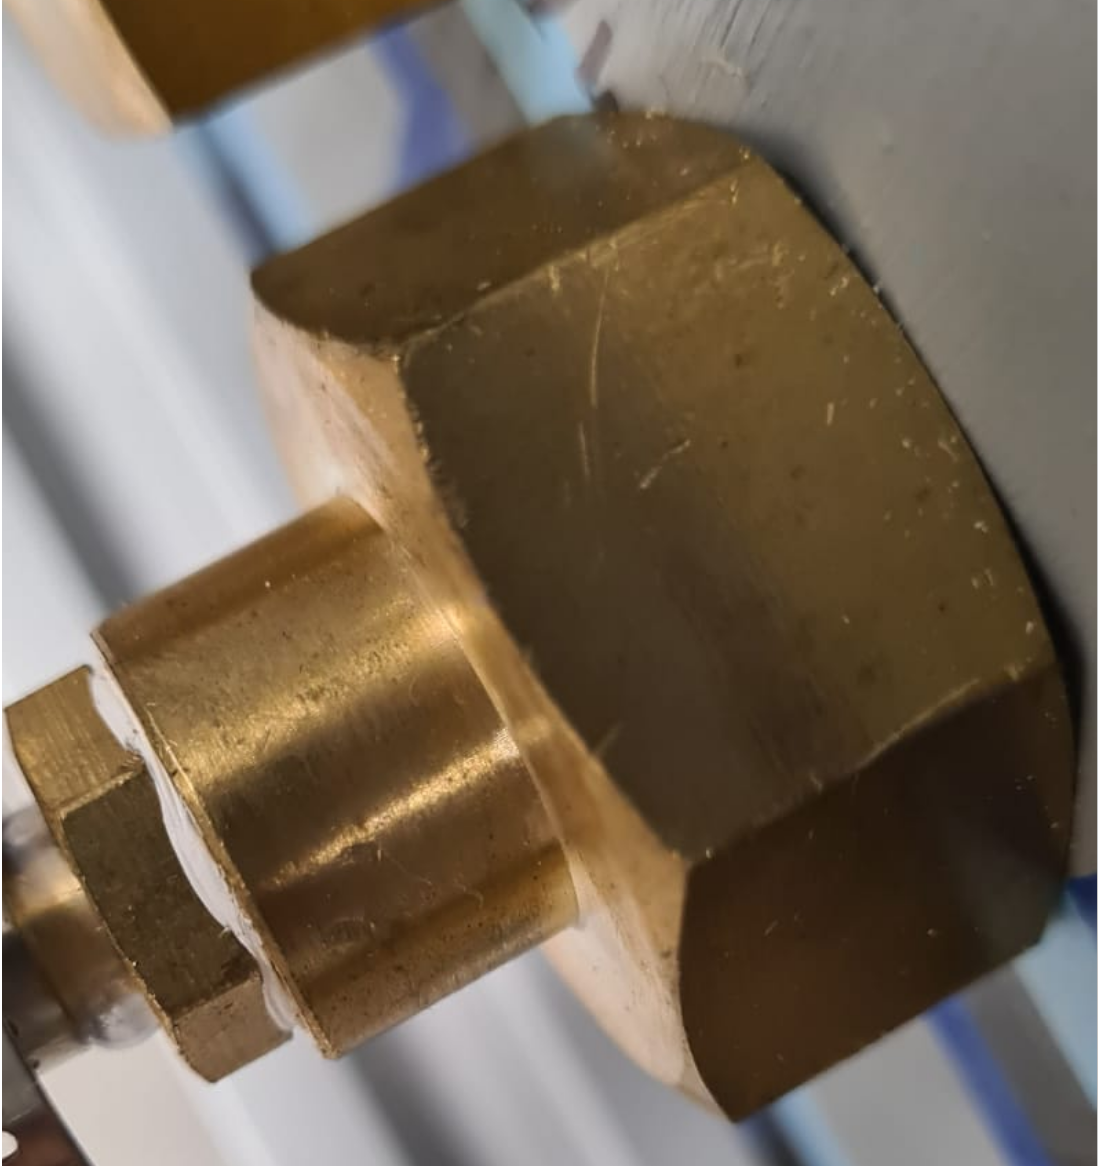
\includegraphics[width=0.3\textwidth]{zu4.}
		\centering
		\caption{Ventile am Gehäuse anbringen. Als Nächstes das Fitting ½ Zoll (DN 15) Innengewinde auf 6 mm Innendurchmesser Schlauch anbringen.}
	\end{figure}
		
	5.
	
	\begin{figure}[htb]
		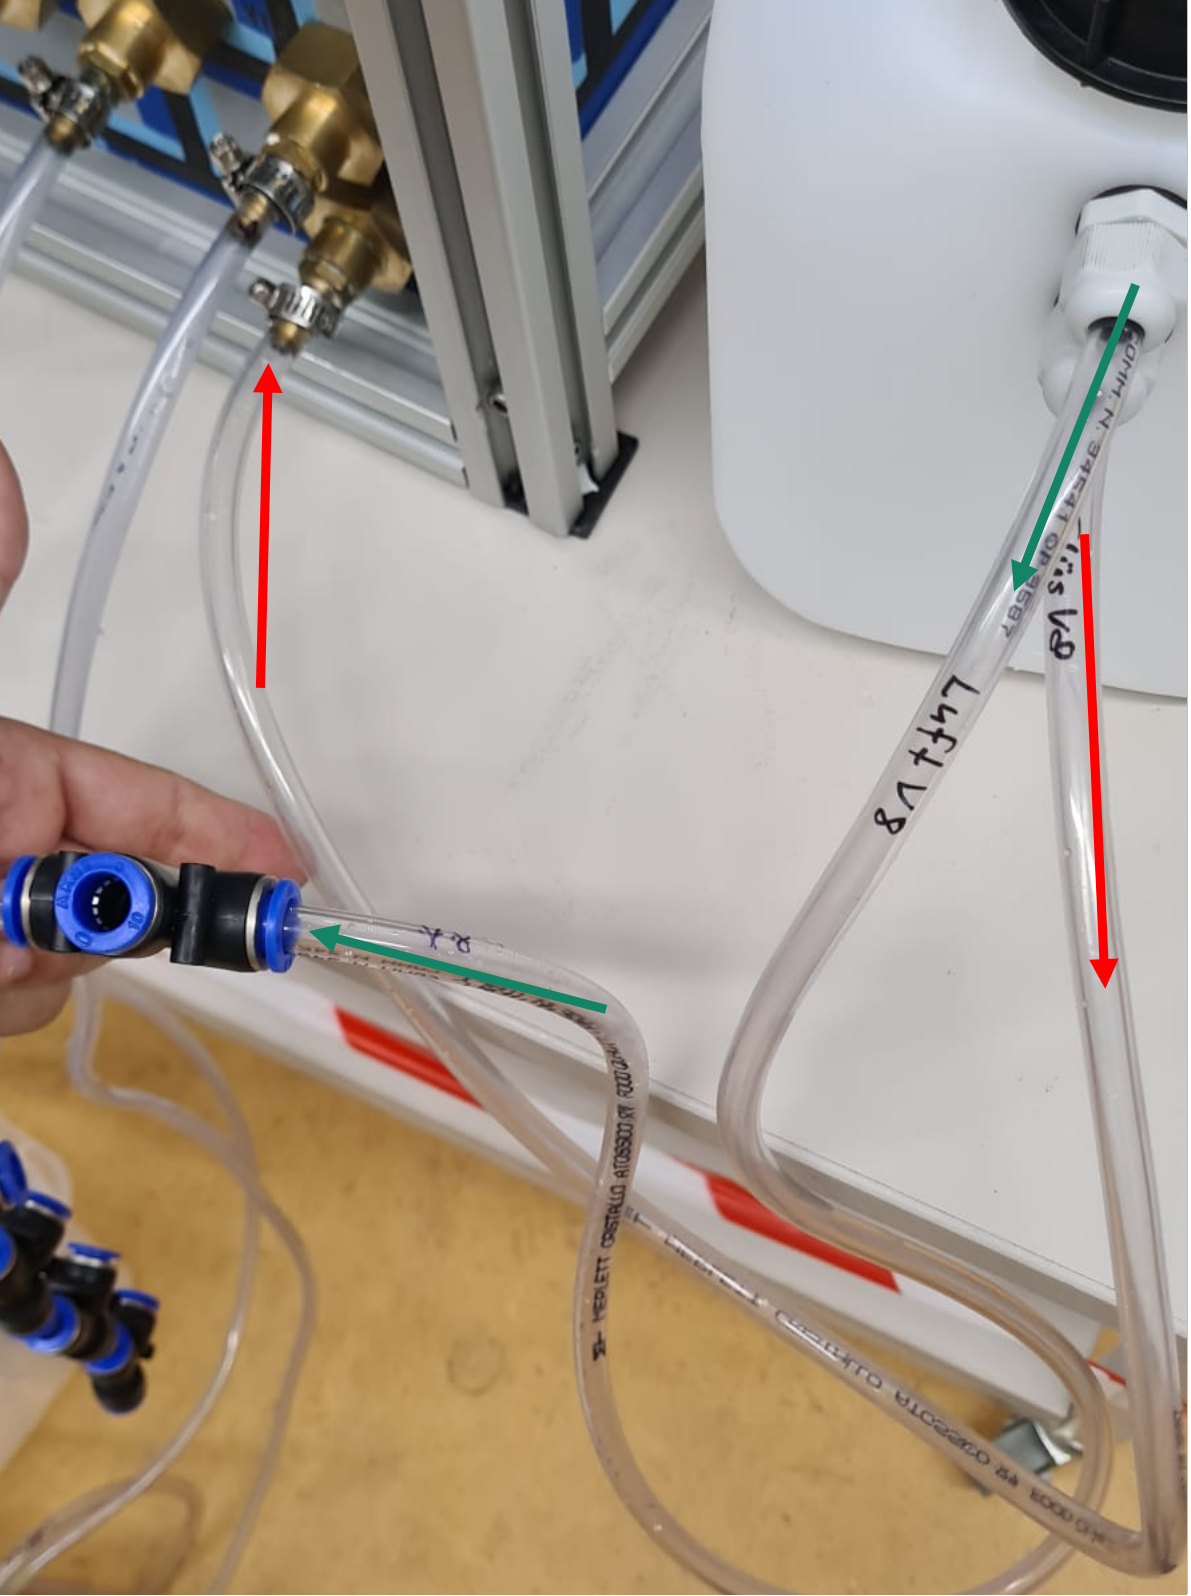
\includegraphics[width=0.4\textwidth]{zu5.}
		\centering
		\caption{Behälter mit Ventilen und T Stücken verbinden.Grün= Luft; Rot=Flüssigkeit}
	\end{figure}
	
	\newpage
	6.
	
	\begin{figure}[htb]
		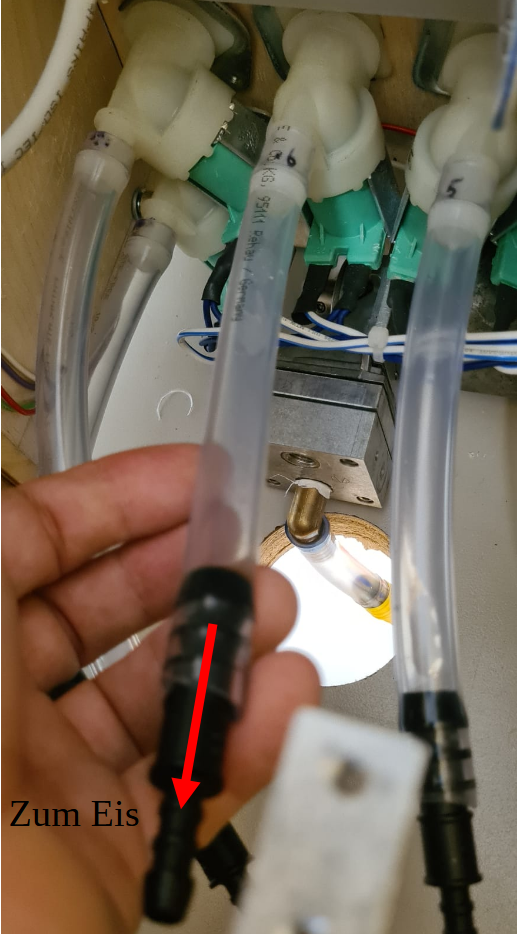
\includegraphics[width=0.4\textwidth]{zu6.}
		\centering
		\caption{Auf der Anderen Seite vom Ventil ca 5 cm langen 10 mm Schlauch anbringen. Anschließend Schlauchverbinder 10 mm auf 6 mm anbringen.}
	\end{figure}
	
	7.
	
	\begin{figure}[htb]
		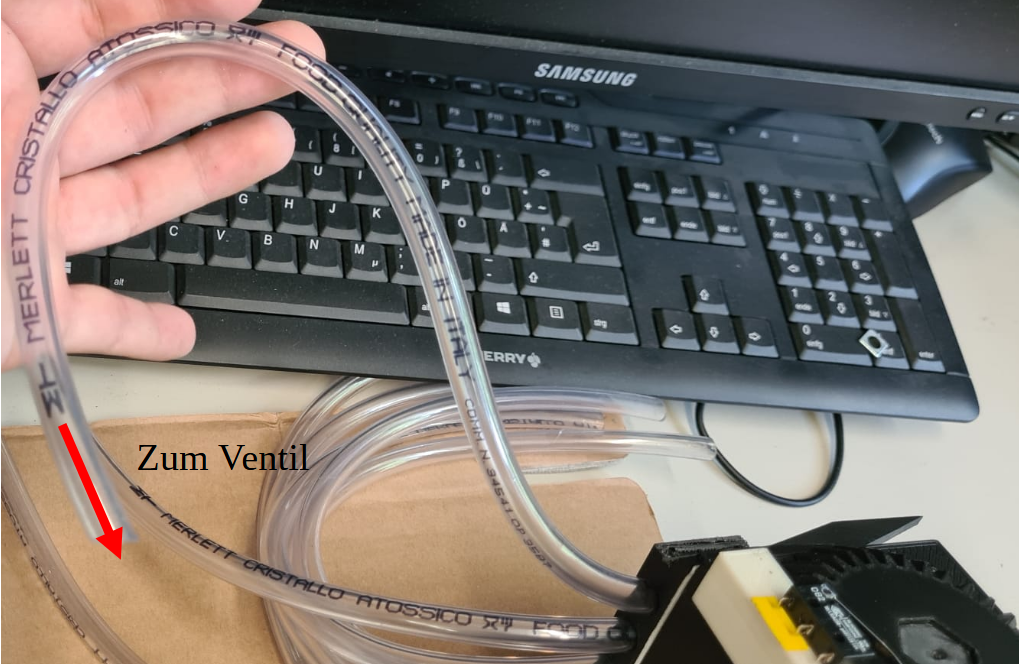
\includegraphics[width=0.6\textwidth]{zu7.}
		\centering
		\caption{Dies muss nur noch mit dem Schlauch vom Eis Verbunden werden.}
	\end{figure}
	\newpage
	8.
	
	\begin{figure}[htb]
		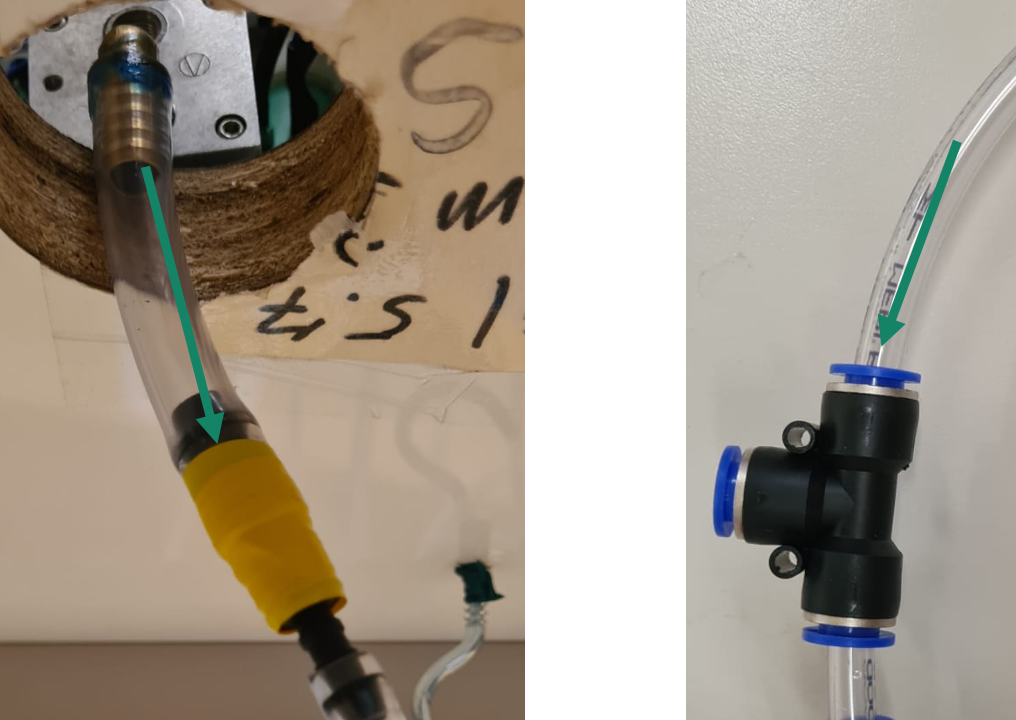
\includegraphics[width=1\textwidth]{zu8.}
		\centering
		\caption{Verbindung der Pumpe zu den T Stücken}
	\end{figure}
	
	

	\chapter{Eisbehälter}
	Der Eisdosierer besteht aus mehreren Komponenten, die zum Großenteil per 3D-Druck gefertigt wurden und wie folgt zusammengefügt werden.\\
	\\
	1.\\	
	Der Aufbewahrungstrichter (a) wird mit dem Gehäuse des Dosierers (b) verklebt, so das die obere Öffnung direkt mit der des Aufbewahrungstrichter übereinstimmt und die vordere Öffnung in Richtung der längeren Trichterschräge zeigt\\
	\\
	2.\\
	Die Dosierwalze (c) wird in das Gehäuse des Dosierers eingeschoben, sodass der Anschluss für das Zahnrad nach rechts zeig.\\
	\\
	3.\\
	Nun werden die Seitenteile (d,e) des Dosierers mit jeweils vier kurzen Schrauben fixiert, dabei sind die Löcher vorzubohren und mit einem größeren Bohrer an zu senken, damit die Schraubenköpfe bündig abschließen und das Zahnrad später besser läuft.\\
	\\
	4.\\
	Jetzt wird das große Zahnrad (f) auf die Walze aufgesteckt.\\
	\\
	5.\\
	Nun folgt die Montage der Endlagenschalter, dafür wird am Rand des Zahnrades eine Schraube montiert, die sich an derselben Position befindet wie die Öffnung des Dosierfaches in der Walze. Danach kann der Haltewinkel (g) befestigt werden, so dass sich die Schräge parallel zu der des Zahnrades befindet, und ein Schalter oberhalb des Zahnrades befindet, wenn Sie von vorne auf das Zahnrad schauen und der andere Teil rechts.\\
	\\
	6.\\
	Der erste Schalter (i) wird so montiert das, wenn er auslöst die das Eis in die Walze fallen kann. Der zweite (j) wird an den andern Teil des Winkels montiert.\\
	\\
	7.\\
	Danach wird der Ausgangstrichter (k) direkt unten an den Dosierer (b) montiert und dabei die zwei kleinen Dreiecke (l) in die Lücke zwischen Dosierer und Trichter geklebt.\\
	\\
	8.
	\\Die Halteschienen (m) für den Spritzschutz werden unten an den Ausgang des Ausgangstrichter (k) geklebt.\\
	\\
	9.\\
	Der obere Teil (n) des Spritzschutzes wird auf den unteren (o) geklebt und in die Halteschienen (m)) geschoben.\\
	\\
	10.\\
	Als letztes wird der Eisdosierer oben in der Maschine befestigt, das kleine Zahnrad auf die Motorwelle geklebt und dieser dann so an der rechten Seitenwand befestigt, dass er das große Zahnrad antreibt.\\
	\newpage
	11.\\
	Zum Schluss wird noch der Verklemmschutz im Aufbewahrungstrichter befestigt das er mittig in die Öffnung ragt.\\
	\\
	\begin{figure}[htb]
		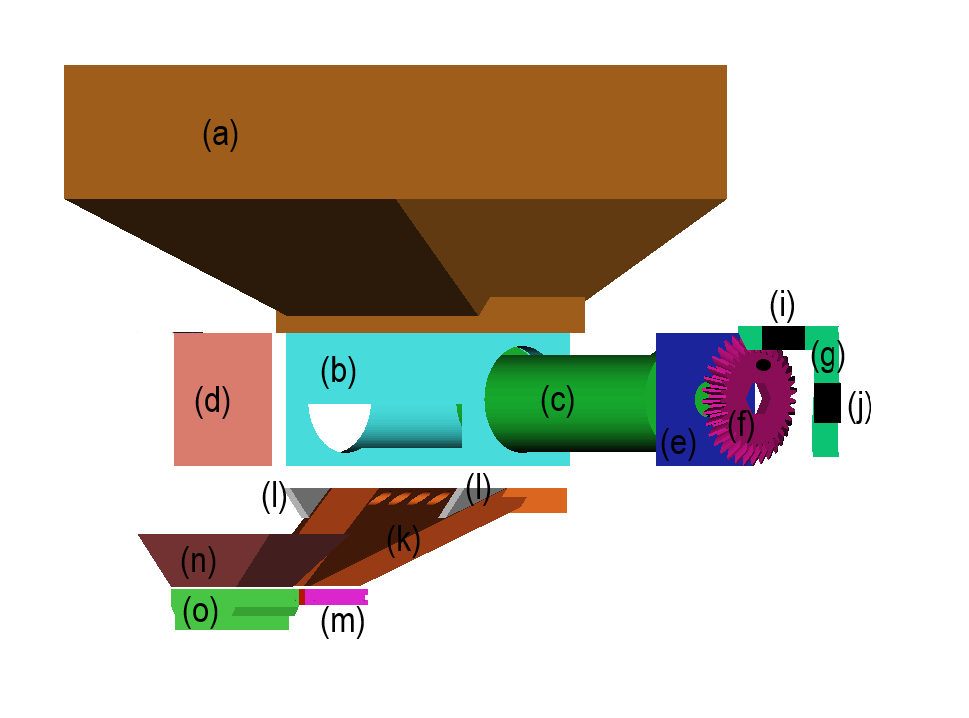
\includegraphics[width=0.6\textwidth]{Explosion2.png}
		\centering
		\caption{Zusammenbau}
	\end{figure}
	\\
	12.\\
	Befestigen Sie die Einheit am oberen Rand des Gehäuses
	
	\chapter{Bildschirmhalterung}
	1.\\
	 Verbinden Sie das Netzwerkkabel und das Holsteckerkabel mit dem Bildschirm\\
	 \\
	 2.\\
	 Setzen Sie den Bildschirm in die Halterung ein und und Sie die Kabel durch die Öffnung am Seitenteil\\
	 \\
	 3.\\
	 Montieren Sie das Seitenteil.\\
	 \\
	 4.\\
	 Verbinden Sie die Bildschirmkabel mit dem Anschluss auf der Rückseite des Gehäuses der Cocktailmaschine
	
	\chapter{SPS-Programm}
	1.\\
	Jetzt wird die Maschine zum ersten Mal mit Energie versorgt\\
	\\
	2.\\
	Installieren Sie das B\&R-Automatisationstudio auf Ihrem PC\\
	\\
	3.\\
	Verbinden Sie die SPS mit Ihrem PC und dem Programm\\
	\\
	4.\\
	Laden Sie das <Sie die fertige Software aus dem Github, auf die SPS\\
	
	\chapter{Schluss}
	Jetzt können Sie die Zutaten in die entsprechenden Behälter füllen, einen Becher einstellen und den Ihren ersten Cocktail auf dem Display auswählen.\\
	[6cm]
	\begin{center}
	\textbf{\huge{Wir wünschen viel Spaß beim \\
	Genießen und Probieren!}}
	\end{center}

	
\end{document}